\documentclass[12pt,a4paper,]{scrartcl}
\usepackage{lmodern}
\usepackage{amssymb,amsmath}
\usepackage{ifxetex,ifluatex}
\usepackage{fixltx2e} % provides \textsubscript
\ifnum 0\ifxetex 1\fi\ifluatex 1\fi=0 % if pdftex
  \usepackage[T1]{fontenc}
  \usepackage[utf8]{inputenc}
\else % if luatex or xelatex
  \ifxetex
    \usepackage{mathspec}
  \else
    \usepackage{fontspec}
  \fi
  \defaultfontfeatures{Ligatures=TeX,Scale=MatchLowercase}
\fi
% use upquote if available, for straight quotes in verbatim environments
\IfFileExists{upquote.sty}{\usepackage{upquote}}{}
% use microtype if available
\IfFileExists{microtype.sty}{%
\usepackage{microtype}
\UseMicrotypeSet[protrusion]{basicmath} % disable protrusion for tt fonts
}{}
\usepackage[margin=1in]{geometry}
\usepackage{hyperref}
\hypersetup{unicode=true,
            pdftitle={Creación eficiente de modelos estadísticos para detección automática y precisa de entidades nombradas},
            pdfauthor={Horacio Miguel Gómez (L:50825); Juan Pablo Orsay (L:49373); Proyecto final de carrera},
            pdfborder={0 0 0},
            breaklinks=true}
\urlstyle{same}  % don't use monospace font for urls
\usepackage{color}
\usepackage{fancyvrb}
\newcommand{\VerbBar}{|}
\newcommand{\VERB}{\Verb[commandchars=\\\{\}]}
\DefineVerbatimEnvironment{Highlighting}{Verbatim}{commandchars=\\\{\}}
% Add ',fontsize=\small' for more characters per line
\usepackage{framed}
\definecolor{shadecolor}{RGB}{248,248,248}
\newenvironment{Shaded}{\begin{snugshade}}{\end{snugshade}}
\newcommand{\AlertTok}[1]{\textcolor[rgb]{0.94,0.16,0.16}{#1}}
\newcommand{\AnnotationTok}[1]{\textcolor[rgb]{0.56,0.35,0.01}{\textbf{\textit{#1}}}}
\newcommand{\AttributeTok}[1]{\textcolor[rgb]{0.77,0.63,0.00}{#1}}
\newcommand{\BaseNTok}[1]{\textcolor[rgb]{0.00,0.00,0.81}{#1}}
\newcommand{\BuiltInTok}[1]{#1}
\newcommand{\CharTok}[1]{\textcolor[rgb]{0.31,0.60,0.02}{#1}}
\newcommand{\CommentTok}[1]{\textcolor[rgb]{0.56,0.35,0.01}{\textit{#1}}}
\newcommand{\CommentVarTok}[1]{\textcolor[rgb]{0.56,0.35,0.01}{\textbf{\textit{#1}}}}
\newcommand{\ConstantTok}[1]{\textcolor[rgb]{0.00,0.00,0.00}{#1}}
\newcommand{\ControlFlowTok}[1]{\textcolor[rgb]{0.13,0.29,0.53}{\textbf{#1}}}
\newcommand{\DataTypeTok}[1]{\textcolor[rgb]{0.13,0.29,0.53}{#1}}
\newcommand{\DecValTok}[1]{\textcolor[rgb]{0.00,0.00,0.81}{#1}}
\newcommand{\DocumentationTok}[1]{\textcolor[rgb]{0.56,0.35,0.01}{\textbf{\textit{#1}}}}
\newcommand{\ErrorTok}[1]{\textcolor[rgb]{0.64,0.00,0.00}{\textbf{#1}}}
\newcommand{\ExtensionTok}[1]{#1}
\newcommand{\FloatTok}[1]{\textcolor[rgb]{0.00,0.00,0.81}{#1}}
\newcommand{\FunctionTok}[1]{\textcolor[rgb]{0.00,0.00,0.00}{#1}}
\newcommand{\ImportTok}[1]{#1}
\newcommand{\InformationTok}[1]{\textcolor[rgb]{0.56,0.35,0.01}{\textbf{\textit{#1}}}}
\newcommand{\KeywordTok}[1]{\textcolor[rgb]{0.13,0.29,0.53}{\textbf{#1}}}
\newcommand{\NormalTok}[1]{#1}
\newcommand{\OperatorTok}[1]{\textcolor[rgb]{0.81,0.36,0.00}{\textbf{#1}}}
\newcommand{\OtherTok}[1]{\textcolor[rgb]{0.56,0.35,0.01}{#1}}
\newcommand{\PreprocessorTok}[1]{\textcolor[rgb]{0.56,0.35,0.01}{\textit{#1}}}
\newcommand{\RegionMarkerTok}[1]{#1}
\newcommand{\SpecialCharTok}[1]{\textcolor[rgb]{0.00,0.00,0.00}{#1}}
\newcommand{\SpecialStringTok}[1]{\textcolor[rgb]{0.31,0.60,0.02}{#1}}
\newcommand{\StringTok}[1]{\textcolor[rgb]{0.31,0.60,0.02}{#1}}
\newcommand{\VariableTok}[1]{\textcolor[rgb]{0.00,0.00,0.00}{#1}}
\newcommand{\VerbatimStringTok}[1]{\textcolor[rgb]{0.31,0.60,0.02}{#1}}
\newcommand{\WarningTok}[1]{\textcolor[rgb]{0.56,0.35,0.01}{\textbf{\textit{#1}}}}
\usepackage{longtable,booktabs}
\usepackage{graphicx}
% grffile has become a legacy package: https://ctan.org/pkg/grffile
\IfFileExists{grffile.sty}{%
\usepackage{grffile}
}{}
\makeatletter
\def\maxwidth{\ifdim\Gin@nat@width>\linewidth\linewidth\else\Gin@nat@width\fi}
\def\maxheight{\ifdim\Gin@nat@height>\textheight\textheight\else\Gin@nat@height\fi}
\makeatother
% Scale images if necessary, so that they will not overflow the page
% margins by default, and it is still possible to overwrite the defaults
% using explicit options in \includegraphics[width, height, ...]{}
\setkeys{Gin}{width=\maxwidth,height=\maxheight,keepaspectratio}
\IfFileExists{parskip.sty}{%
\usepackage{parskip}
}{% else
\setlength{\parindent}{0pt}
\setlength{\parskip}{6pt plus 2pt minus 1pt}
}
\setlength{\emergencystretch}{3em}  % prevent overfull lines
\providecommand{\tightlist}{%
  \setlength{\itemsep}{0pt}\setlength{\parskip}{0pt}}
\setcounter{secnumdepth}{5}
% Redefines (sub)paragraphs to behave more like sections
\ifx\paragraph\undefined\else
\let\oldparagraph\paragraph
\renewcommand{\paragraph}[1]{\oldparagraph{#1}\mbox{}}
\fi
\ifx\subparagraph\undefined\else
\let\oldsubparagraph\subparagraph
\renewcommand{\subparagraph}[1]{\oldsubparagraph{#1}\mbox{}}
\fi

%%% Use protect on footnotes to avoid problems with footnotes in titles
\let\rmarkdownfootnote\footnote%
\def\footnote{\protect\rmarkdownfootnote}

%%% Change title format to be more compact
\usepackage{titling}

% Create subtitle command for use in maketitle
\providecommand{\subtitle}[1]{
  \posttitle{
    \begin{center}\large#1\end{center}
    }
}

\setlength{\droptitle}{-2em}

  \title{Creación eficiente de modelos estadísticos para detección automática y precisa de entidades nombradas}
    \pretitle{\vspace{\droptitle}\centering\huge}
  \posttitle{\par}
  \subtitle{Instituto Tecnológico de Buenos Aires}
  \author{Horacio Miguel Gómez \((L:50825)\) \\ Juan Pablo Orsay \((L:49373)\) \\ Proyecto final de carrera}
    \preauthor{\centering\large\emph}
  \postauthor{\par}
      \predate{\centering\large\emph}
  \postdate{\par}
    \date{2019-11-20}

% Usefull information about documentclass
% http://ctan.dcc.uchile.cl/macros/latex/contrib/koma-script/doc/scrguien.pdf

\usepackage[spanish]{babel} % español

\usepackage{fontspec} % xelatexfont
\defaultfontfeatures[TeX Gyre Adventor]
{
  Extension      = .otf,
  UprightFont    = texgyreadventor-regular,
  BoldFont       = texgyreadventor-bold,
  ItalicFont     = texgyreadventor-italic,
  BoldItalicFont = texgyreadventor-bolditalic,
}
\setmainfont{TeX Gyre Adventor}

\usepackage{booktabs}
\usepackage{amsthm}
% \usepackage{biblatex}

%\usepackage{hyperref} % for links between refs
%\hypersetup{
%    colorlinks = true % ref links,
%    linkcolor=\color{Maroon},
%    urlcolor=\color{Maroon}
%}

\usepackage[hypcap=true, labelfont=bf]{caption} % ref links point to top of images instead of caption
\usepackage{float} % for images with H

\usepackage{csquotes} % for quoting
% Don't use xcolor (bug with bookdown).
% Define them instead. http://latexcolor.com/
\definecolor{slategray}{rgb}{0.44, 0.5, 0.56}
\AtBeginEnvironment{quote}{\color{slategray}}

% \BeforeBeginEnvironment{tableofcontents}{\pagebreak}
% \AfterEndEnvironment{tableofcontents}{\pagebreak}

\usepackage{lastpage} % to get the last page
\usepackage{scrlayer-scrpage} % Control of page headers and footers with KOMA documentclass
\cfoot{\thepage\ de \pageref{LastPage}}
\ohead{Instituto Tecnológico de Buenos Aires \linebreak Proyecto Final - Gomez, Orsay}
\pagestyle{scrheadings}

\makeatletter
\def\thm@space@setup{
  \thm@preskip=8pt plus 2pt minus 4pt
  \thm@postskip=\thm@preskip
}
\makeatother

\begin{document}
\maketitle

{
\setcounter{tocdepth}{2}
\tableofcontents
}
\newpage

\hypertarget{abstract}{%
\section*{\texorpdfstring{\emph{Abstract}}{Abstract}}\label{abstract}}
\addcontentsline{toc}{section}{\emph{Abstract}}

\begin{quote}
TODO: escribir abstract
\end{quote}

\hypertarget{intro}{%
\section{Introducción}\label{intro}}

\hypertarget{state-of-art}{%
\section{Estado del arte}\label{state-of-art}}

\hypertarget{el-naive-approach}{%
\subsection{\texorpdfstring{El \enquote{naive approach}}{El ``naive approach''}}\label{el-naive-approach}}

tagueo con expresiones regulares\ldots{}

\hypertarget{redes-neuronales-y-modelos-estaduxedsticos}{%
\subsection{Redes neuronales y modelos estadísticos}\label{redes-neuronales-y-modelos-estaduxedsticos}}

Redes neuronales convolucionales
\url{https://es.wikipedia.org/wiki/Redes_neuronales_convolucionales}

\hypertarget{la-formula-para-deep-learning}{%
\subsection{\texorpdfstring{La formula para \enquote{deep-learning}}{La formula para ``deep-learning''}}\label{la-formula-para-deep-learning}}

articulo spacy

\hypertarget{embed}{%
\subsubsection{embed}\label{embed}}

\begin{figure}[H]

{\centering 
\includegraphics{assets/deep-learning-formula-nlp_embed.pdf} 

}

\caption{TODO: embed}\label{fig:formula-embed}
\end{figure}

\hypertarget{encode}{%
\subsubsection{encode}\label{encode}}

\begin{figure}[H]

{\centering 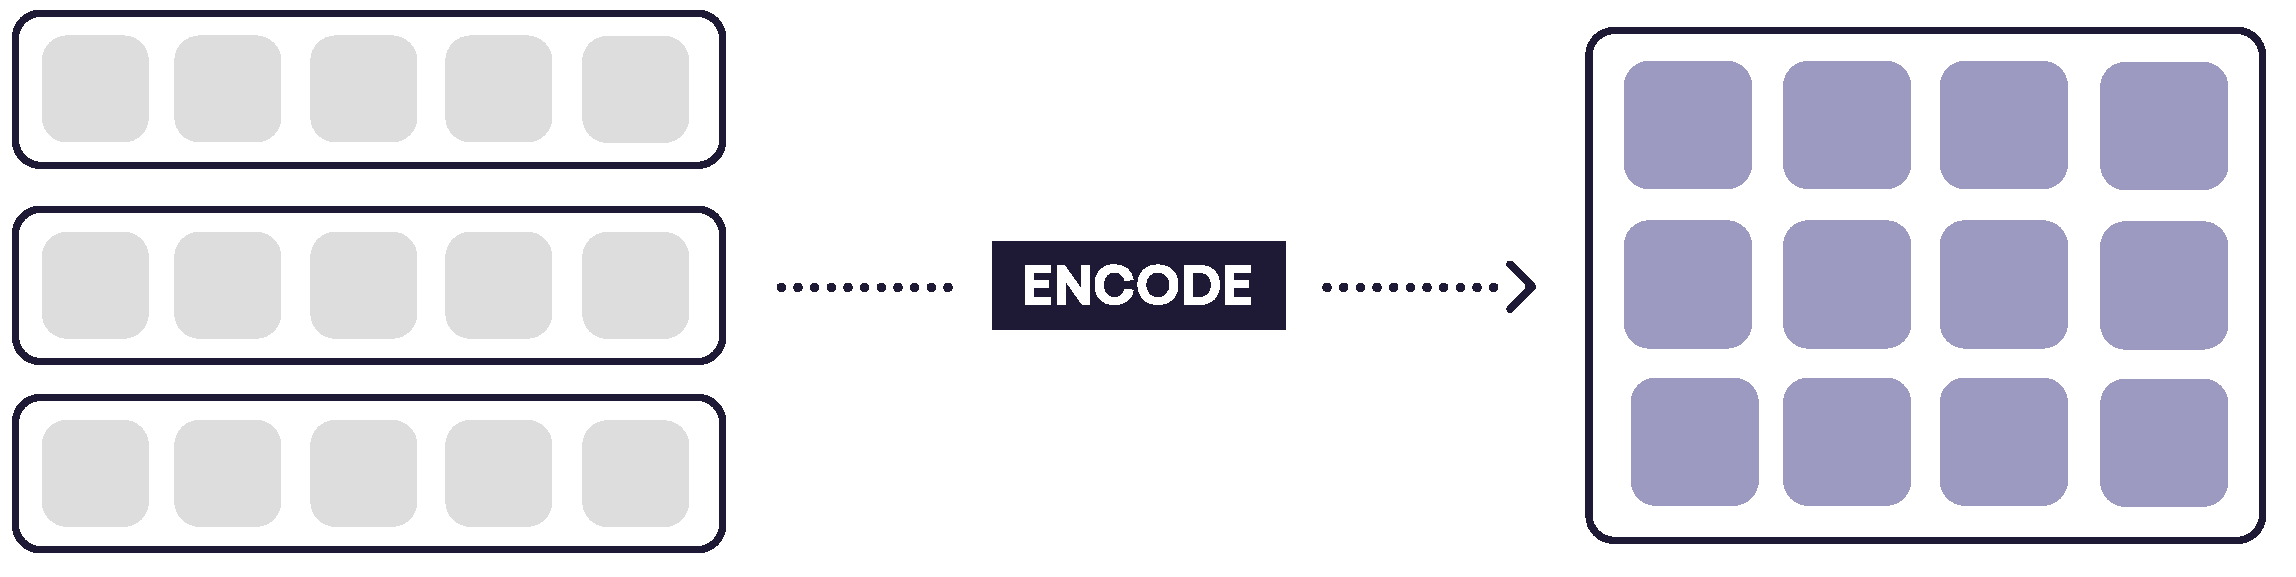
\includegraphics{assets/deep-learning-formula-nlp_encode.pdf} 

}

\caption{TODO: encode}\label{fig:formula-encode}
\end{figure}

\hypertarget{attend}{%
\subsubsection{attend}\label{attend}}

\begin{figure}[H]

{\centering 
\includegraphics{assets/deep-learning-formula-nlp_attend.pdf} 

}

\caption{TODO: attend}\label{fig:formula-attend}
\end{figure}

\hypertarget{predict}{%
\subsubsection{predict}\label{predict}}

\begin{figure}[H]

{\centering 
\includegraphics{assets/deep-learning-formula-nlp_predict.pdf} 

}

\caption{TODO: predict}\label{fig:formula-predict}
\end{figure}

Here is a review of existing methods.

\hypertarget{statistical-entity-recognition-model}{%
\subsection{statistical entity recognition model}\label{statistical-entity-recognition-model}}

\hypertarget{word-vectors}{%
\subsection{Word vectors}\label{word-vectors}}

\[\vec{king} - \vec{man} + \vec{woman} \approx \vec{queen}\]

(Ethayarajh, Duvenaud, \& Hirst, \protect\hyperlink{ref-ethayarajh-etal-2019-towards}{2019})

\begin{figure}[H]

{\centering 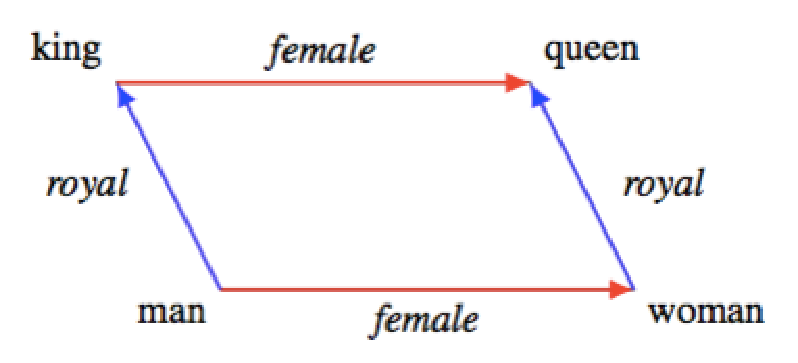
\includegraphics{assets/parallelogram.pdf} 

}

\caption{Parallelogram structure in the vector space (by definition)}\label{fig:vec-parallelogram}
\end{figure}

\url{https://www.youtube.com/watch?v=sqDHBH9IjRU}
SPACY'S ENTITY RECOGNITION MODEL: incremental parsing with Bloom embeddings \& residual CNNs

\url{https://github.com/explosion/talks/blob/master/2017-11-02_Practical-and-Effective-Neural-NER.pdf}
\url{https://github.com/explosion/talks/blob/master/2018-04-12_Embed-Encode-Attend-Predict.pdf}

\hypertarget{problem-definition}{%
\section{Definición del problema}\label{problem-definition}}

El bottleneck en AI es la data, no los algoritmos.
quote de: \url{https://github.com/explosion/talks/blob/master/2016-11-28_The-State-of-AI-2016.pdf}

\url{https://github.com/explosion/talks/blob/master/2018-04-12_Embed-Encode-Attend-Predict.pdf}

\hypertarget{implementation}{%
\section{NERd (Implementación)}\label{implementation}}

Definido el problema, queda claro que la creación de un modelo entrenado es de vital importancia para cualquier problema de tagueo de entidades.
Es por ello que en el presente proyecto final hemos creado una herramienta para el entrenamiento eficiente de modelos estadísticos así como también una interfaz y API para poder consultar entidades.
El nombre de esta herramienta es \textbf{NERd}, sigla cuyo significado en inglés es \emph{\textbf{N}amed \textbf{E}ntity \textbf{R}ecognition \textbf{D}uh}\footnote{Expresión de obviedad. \emph{Used to express your belief that what was said was extremely obvious} (``Duh definition,'' \protect\hyperlink{ref-cambridge_duh}{2019})}!

Para organizar este capítulo vamos a realizar una descripción basada en el modelo de vistas de arquitectura 4+1.

\begin{figure}[H]

{\centering 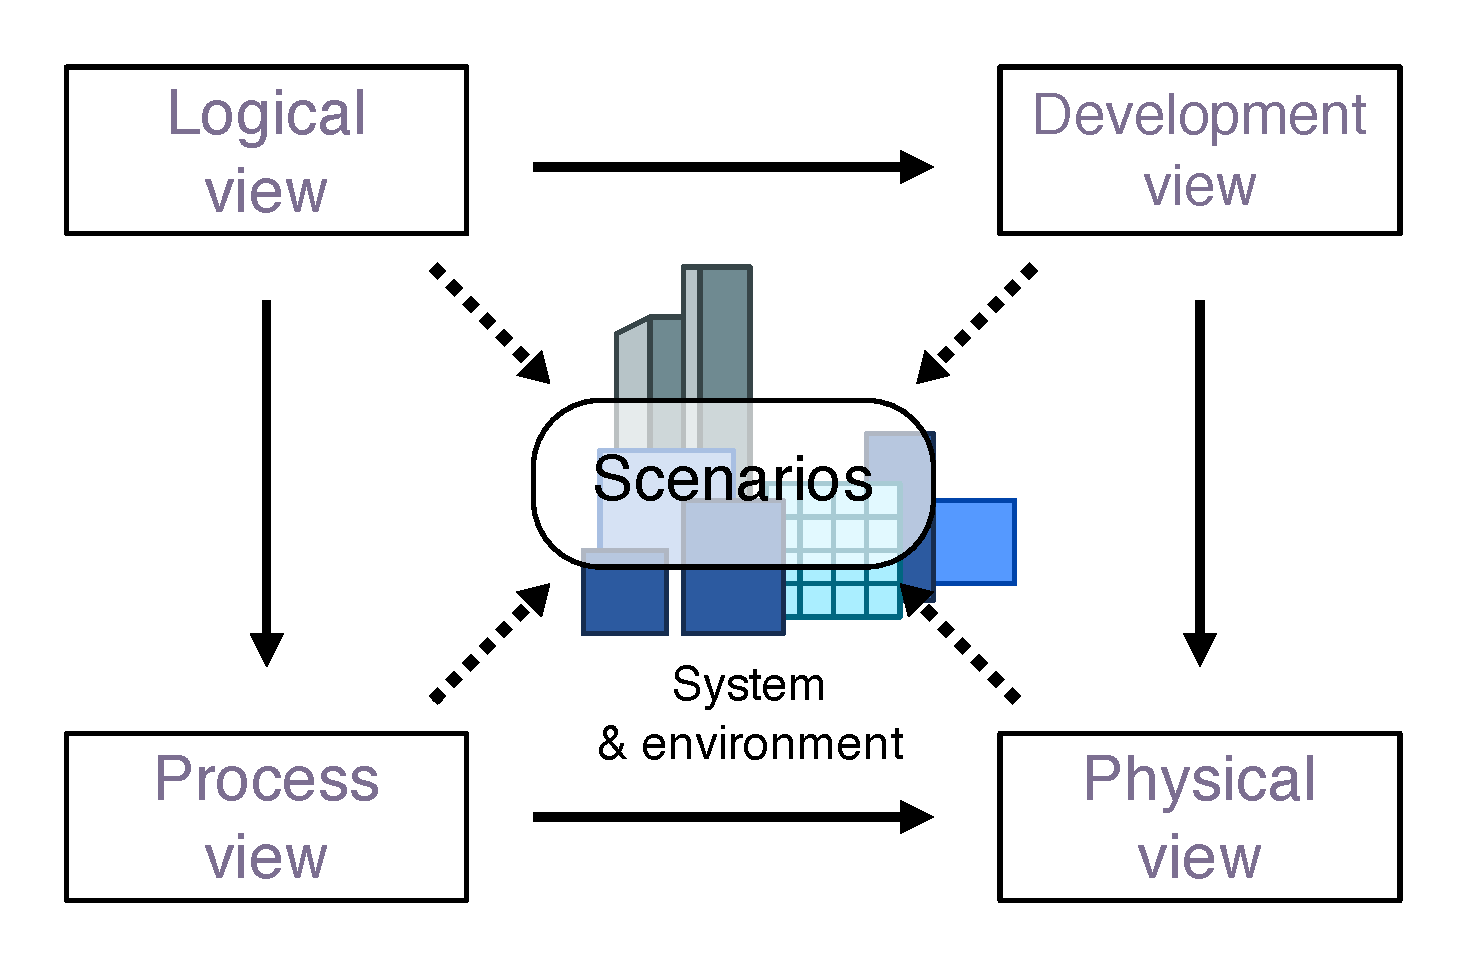
\includegraphics{assets/4+1_Architectural_View_Model.pdf} 

}

\caption{Ilustración de arquitectura 4+1}\label{fig:arq41}
\end{figure}

Este modelo nos permite describir la aplicación de una manera genérica y ordenada.

\begin{quote}
\emph{The \enquote{4+1} view model is rather \enquote{generic}: other notations and tools can be used, other design methods can be used, especially for the logical and process decompositions, but we have indicated the ones we have used with success.}

\hfill --- (Kruchten, \protect\hyperlink{ref-Kruchten:1995:VMA:624610.625529}{1995})
\end{quote}

\hypertarget{vista-luxf3gica}{%
\subsection{Vista lógica}\label{vista-luxf3gica}}

\begin{quote}
La vista lógica se refiere a la funcionalidad que el sistema proporciona a los usuarios finales.
\end{quote}

A continuación detallamos distintas partes del servicio NERd así como también de la interfaz de entrenamiento.

\hypertarget{servicio}{%
\subsubsection{Servicio}\label{servicio}}

El acceso al servicio se realiza mediante un API REST que se auto-documenta debido a implementar la especificación de OpenAPI. A continuación detallamos los endpoints.

\hypertarget{autenticaciuxf3n}{%
\paragraph{Autenticación}\label{autenticaciuxf3n}}

Rutas del API dedicadas a la autenticación de usuarios.

\begin{itemize}
\tightlist
\item
  \textbf{POST} \emph{/api/auth/register}

  \begin{itemize}
  \tightlist
  \item
    Registrar un usuario nuevo.
  \end{itemize}
\item
  \textbf{POST} \emph{/api/auth/token}

  \begin{itemize}
  \tightlist
  \item
    Genera un nuevo token de acceso y refresco con credenciales.
  \item
    Utilizado para la funcionalidad de \emph{login}
  \end{itemize}
\item
  \textbf{POST} \emph{/api/auth/refresh}

  \begin{itemize}
  \tightlist
  \item
    Refresca el token de acceso.
  \item
    Utilizado cuando un token de acceso caducó.
  \end{itemize}
\end{itemize}

\hypertarget{usuarios}{%
\paragraph{Usuarios}\label{usuarios}}

Conjunto de operaciones relacionadas con los usuarios del sistema.

\begin{itemize}
\tightlist
\item
  \textbf{GET} \emph{/api/users}

  \begin{itemize}
  \tightlist
  \item
    Lista de usuarios existentes
  \item
    Separa los resultados en páginas
  \end{itemize}
\item
  \textbf{GET} \emph{/api/users/top5}

  \begin{itemize}
  \tightlist
  \item
    Lista de los 5 usuarios con más entrenamientos
  \end{itemize}
\item
  \textbf{GET} \emph{/api/users/me}

  \begin{itemize}
  \tightlist
  \item
    Retorna la información del usuario logueado
  \end{itemize}
\item
  \textbf{PATCH} \emph{/api/users/me}

  \begin{itemize}
  \tightlist
  \item
    Actualiza la información del usuario logueado
  \end{itemize}
\item
  \textbf{GET} \emph{/api/users/me/trainings}

  \begin{itemize}
  \tightlist
  \item
    Retorna los entrenamientos del usuario logueado
  \item
    Separa los resultados en páginas
  \end{itemize}
\item
  \textbf{GET} \emph{/api/users/\{user\_id\}}

  \begin{itemize}
  \tightlist
  \item
    Retorna la información del usuario especificado por \emph{user\_id}
  \end{itemize}
\item
  \textbf{PATCH} \emph{/api/users/\{user\_id\}}

  \begin{itemize}
  \tightlist
  \item
    Actualiza la información del usuario especificado por \emph{user\_id}
  \end{itemize}
\item
  \textbf{DELETE} \emph{/api/users/\{user\_id\}}

  \begin{itemize}
  \tightlist
  \item
    Borra al usuario especificado por \emph{user\_id}
  \end{itemize}
\item
  \textbf{GET} \_/api/users/\{user\_id\}/trainings

  \begin{itemize}
  \tightlist
  \item
    Retorna los entrenamientos del usuario especificado
  \end{itemize}
\end{itemize}

\hypertarget{roles}{%
\paragraph{Roles}\label{roles}}

\begin{itemize}
\tightlist
\item
  \textbf{GET} \emph{/api/roles}

  \begin{itemize}
  \tightlist
  \item
    Retorna la lista de todos los roles asignables a usuarios del sistema
  \end{itemize}
\end{itemize}

\hypertarget{corpus}{%
\paragraph{Corpus}\label{corpus}}

Rutas dedicadas a operaciones con el corpus del sistema.

\begin{itemize}
\tightlist
\item
  \textbf{GET} \emph{/api/corpus/\{text\_id\}}

  \begin{itemize}
  \tightlist
  \item
    Retorna los detalles del texto especificado por \emph{text\_id}
  \end{itemize}
\item
  \textbf{DELETE} \emph{/api/corpus/\{text\_id\}}

  \begin{itemize}
  \tightlist
  \item
    Borra un texto especificado por \emph{text\_id} del corpus
  \end{itemize}
\item
  \textbf{GET} \emph{/api/corpus/\{text\_id\}/trainings}

  \begin{itemize}
  \tightlist
  \item
    Retorna la lista de entrenamientos proporcionados por los usuarios sobre las entidades en el texto
  \end{itemize}
\item
  \textbf{PUT} \emph{/api/corpus/\{text\_id\}/trainings}

  \begin{itemize}
  \tightlist
  \item
    Agrega un entrenamiento para el texto con id \emph{text\_id}
  \end{itemize}
\item
  \textbf{POST} \emph{/api/corpus/upload}

  \begin{itemize}
  \tightlist
  \item
    Permite agregar textos de manera masiva al sistema
  \item
    Acepta una lista de archivos .txt donde cada línea es un texto a agregar
  \item
    Los archivos deben ser UTF-8
  \end{itemize}
\item
  \textbf{GET} \emph{/api/corpus}

  \begin{itemize}
  \tightlist
  \item
    Lista de textos cargados en el sistema para entrenamiento
  \item
    Separa los resultados en páginas
  \end{itemize}
\item
  \textbf{POST} \emph{/api/corpus}

  \begin{itemize}
  \tightlist
  \item
    Agrega un texto al sistema para entrenamiento
  \end{itemize}
\end{itemize}

\hypertarget{snapshots}{%
\paragraph{Snapshots}\label{snapshots}}

Conjunto de operaciones relacionadas con los snapshots y workers.

\begin{itemize}
\tightlist
\item
  \textbf{GET} \emph{/api/snapshots}

  \begin{itemize}
  \tightlist
  \item
    Listado de los snapshots disponibles
  \item
    Separa los resultados en páginas
  \end{itemize}
\item
  \textbf{GET} \emph{/api/snapshots/\{snapshot\_id\}}

  \begin{itemize}
  \tightlist
  \item
    Retorna información (tipos de entidades, fecha de creación, fecha de entrenamiento, etc.) sobre un snapshot específico
  \end{itemize}
\item
  \textbf{DELETE} \emph{/api/snapshots/\{snapshot\_id\}}

  \begin{itemize}
  \tightlist
  \item
    Borra un snapshot con el id especificado
  \end{itemize}
\item
  \textbf{POST} \emph{/api/snapshots/\{snapshot\_id\}/force-train}

  \begin{itemize}
  \tightlist
  \item
    Envía la tarea de entrenamiento a los workers que tienen el snapshot \emph{snapshot\_id} cargado.
  \end{itemize}
\item
  \textbf{POST} \emph{/api/snapshots/\{snapshot\_id\}/force-untrain}

  \begin{itemize}
  \tightlist
  \item
    Envía la tarea de desentrenar a los workers que tienen el snapshot \emph{snapshot\_id} cargado.
  \end{itemize}
\item
  \textbf{GET} \emph{/api/snapshots/current}

  \begin{itemize}
  \tightlist
  \item
    Retorna información sobre el snapshot actual
  \end{itemize}
\item
  \textbf{PUT} \emph{/api/snapshots/current}

  \begin{itemize}
  \tightlist
  \item
    Crea un nuevo snapshot con la información provista
  \end{itemize}
\end{itemize}

\hypertarget{reconocimiento-de-entidades-nombradas}{%
\paragraph{Reconocimiento de Entidades Nombradas}\label{reconocimiento-de-entidades-nombradas}}

Conjunto de operaciones relacionadas al \emph{Reconocimiento de Entidades Nombradas}

\begin{itemize}
\tightlist
\item
  \textbf{GET} \emph{/api/ner/train}

  \begin{itemize}
  \tightlist
  \item
    Retorna un texto para que un usuario del sistema revise si está correctamente inferido
  \item
    Únicamente retorna textos que el usuario logueado no haya corregido ya
  \end{itemize}
\item
  \textbf{GET} \emph{/api/ner/compare/\{first\_snapshot\}/\{second\_snapshot\}}

  \begin{itemize}
  \tightlist
  \item
    Compara el \emph{Reconocimiento de Entidades Nombradas} entre dos snapshots distintos
  \end{itemize}
\item
  \textbf{POST} \emph{/api/ner/current/parse}

  \begin{itemize}
  \tightlist
  \item
    Retorna un documento Spacy para un texto dado utilizando el snapshot actual
  \end{itemize}
\item
  \textbf{POST} \emph{/api/ner/\{snapshot\_id\}/parse}

  \begin{itemize}
  \tightlist
  \item
    Retorna un documento Spacy para un texto dado utilizando el snapshot especificado
  \end{itemize}
\item
  \textbf{POST} \emph{/api/ner/current/entities}

  \begin{itemize}
  \tightlist
  \item
    Retorna la lista de \emph{Entidades Nombradas} para un texto dado utilizando el modelo actual
  \end{itemize}
\item
  \textbf{POST} \emph{/api/ner/\{snapshot\_id\}/entities}

  \begin{itemize}
  \tightlist
  \item
    Retorna la lista de \emph{Entidades Nombradas} para un texto dado utilizando el modelo especificado
  \end{itemize}
\end{itemize}

\hypertarget{entrenamientos}{%
\paragraph{Entrenamientos}\label{entrenamientos}}

\begin{itemize}
\tightlist
\item
  \textbf{DELETE} \emph{/api/trainings/\{training\_id\}}

  \begin{itemize}
  \tightlist
  \item
    Borra un entrenamiento
  \end{itemize}
\end{itemize}

\hypertarget{workers}{%
\paragraph{Workers}\label{workers}}

\begin{itemize}
\tightlist
\item
  \textbf{GET} \emph{/api/workers/}

  \begin{itemize}
  \tightlist
  \item
    Lista de los workers disponibles
  \end{itemize}
\item
  \textbf{POST} \emph{/api/workers/reassign}

  \begin{itemize}
  \tightlist
  \item
    Reasigna un trabajador de un a versión de snapshot a otra
  \end{itemize}
\end{itemize}

\hypertarget{web}{%
\subsubsection{Web}\label{web}}

La página web de \emph{NERd} está enfocada en las tareas de mantenimiento de los servicios ofrecidos por el \emph{API} así como también ofrece de interfaces que permiten a usuarios del sistema corregir de manera eficiente el modelo de inferencia.

\hypertarget{inicio}{%
\paragraph{Inicio}\label{inicio}}

Pantalla de inicio donde se encuentran accesos rápidos para entrenar el modelo o para poder buscar entidades en textos.
También se encuentra aquí una lista de los 5 usuarios que más contribuyeron a entrenar el modelo. Detrás de esta funcionalidad se busca generar un espíritu competitivo entre los usuarios para que los mismos busquen contribuir más.

\begin{figure}[H]

{\centering 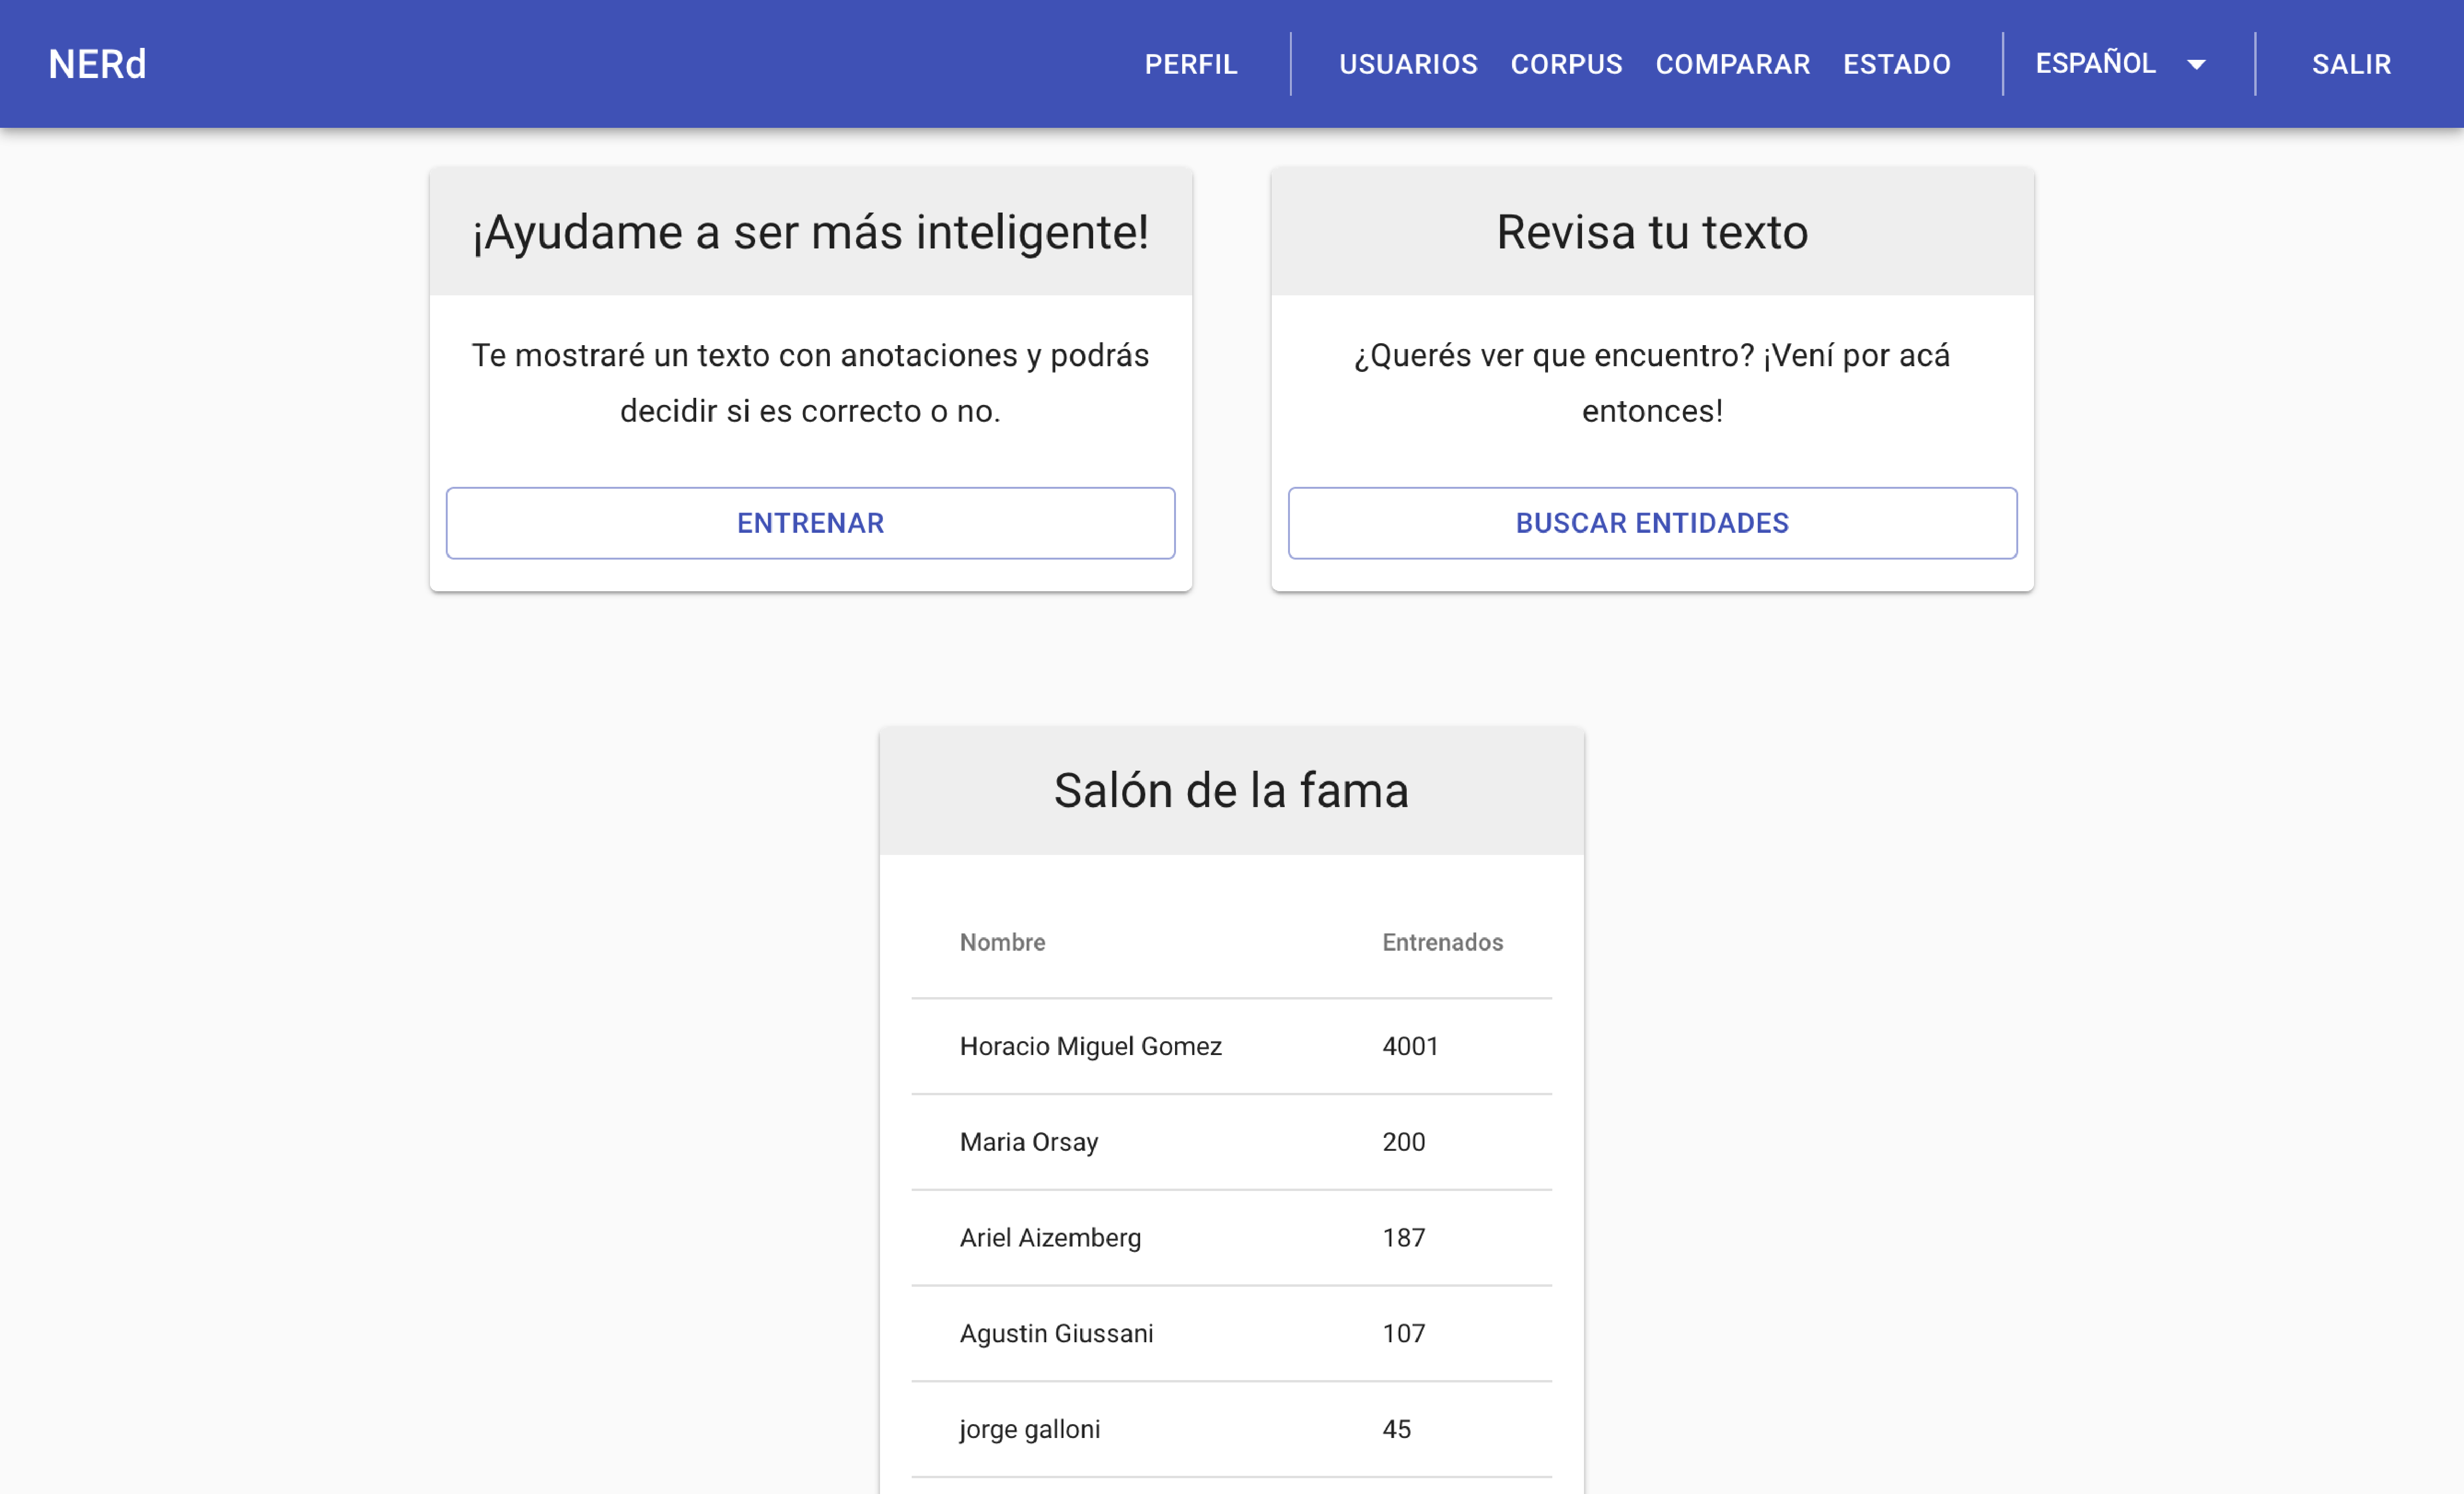
\includegraphics{assets/logic/home-logged-all.pdf} 

}

\caption{Pantalla de inicio con usuario logueado}\label{fig:logic-home}
\end{figure}

Si la persona no cuenta con permisos de entrenador, se le sugiere que contacte a un administrador para que le otorgue el permiso.

\begin{figure}[H]

{\centering 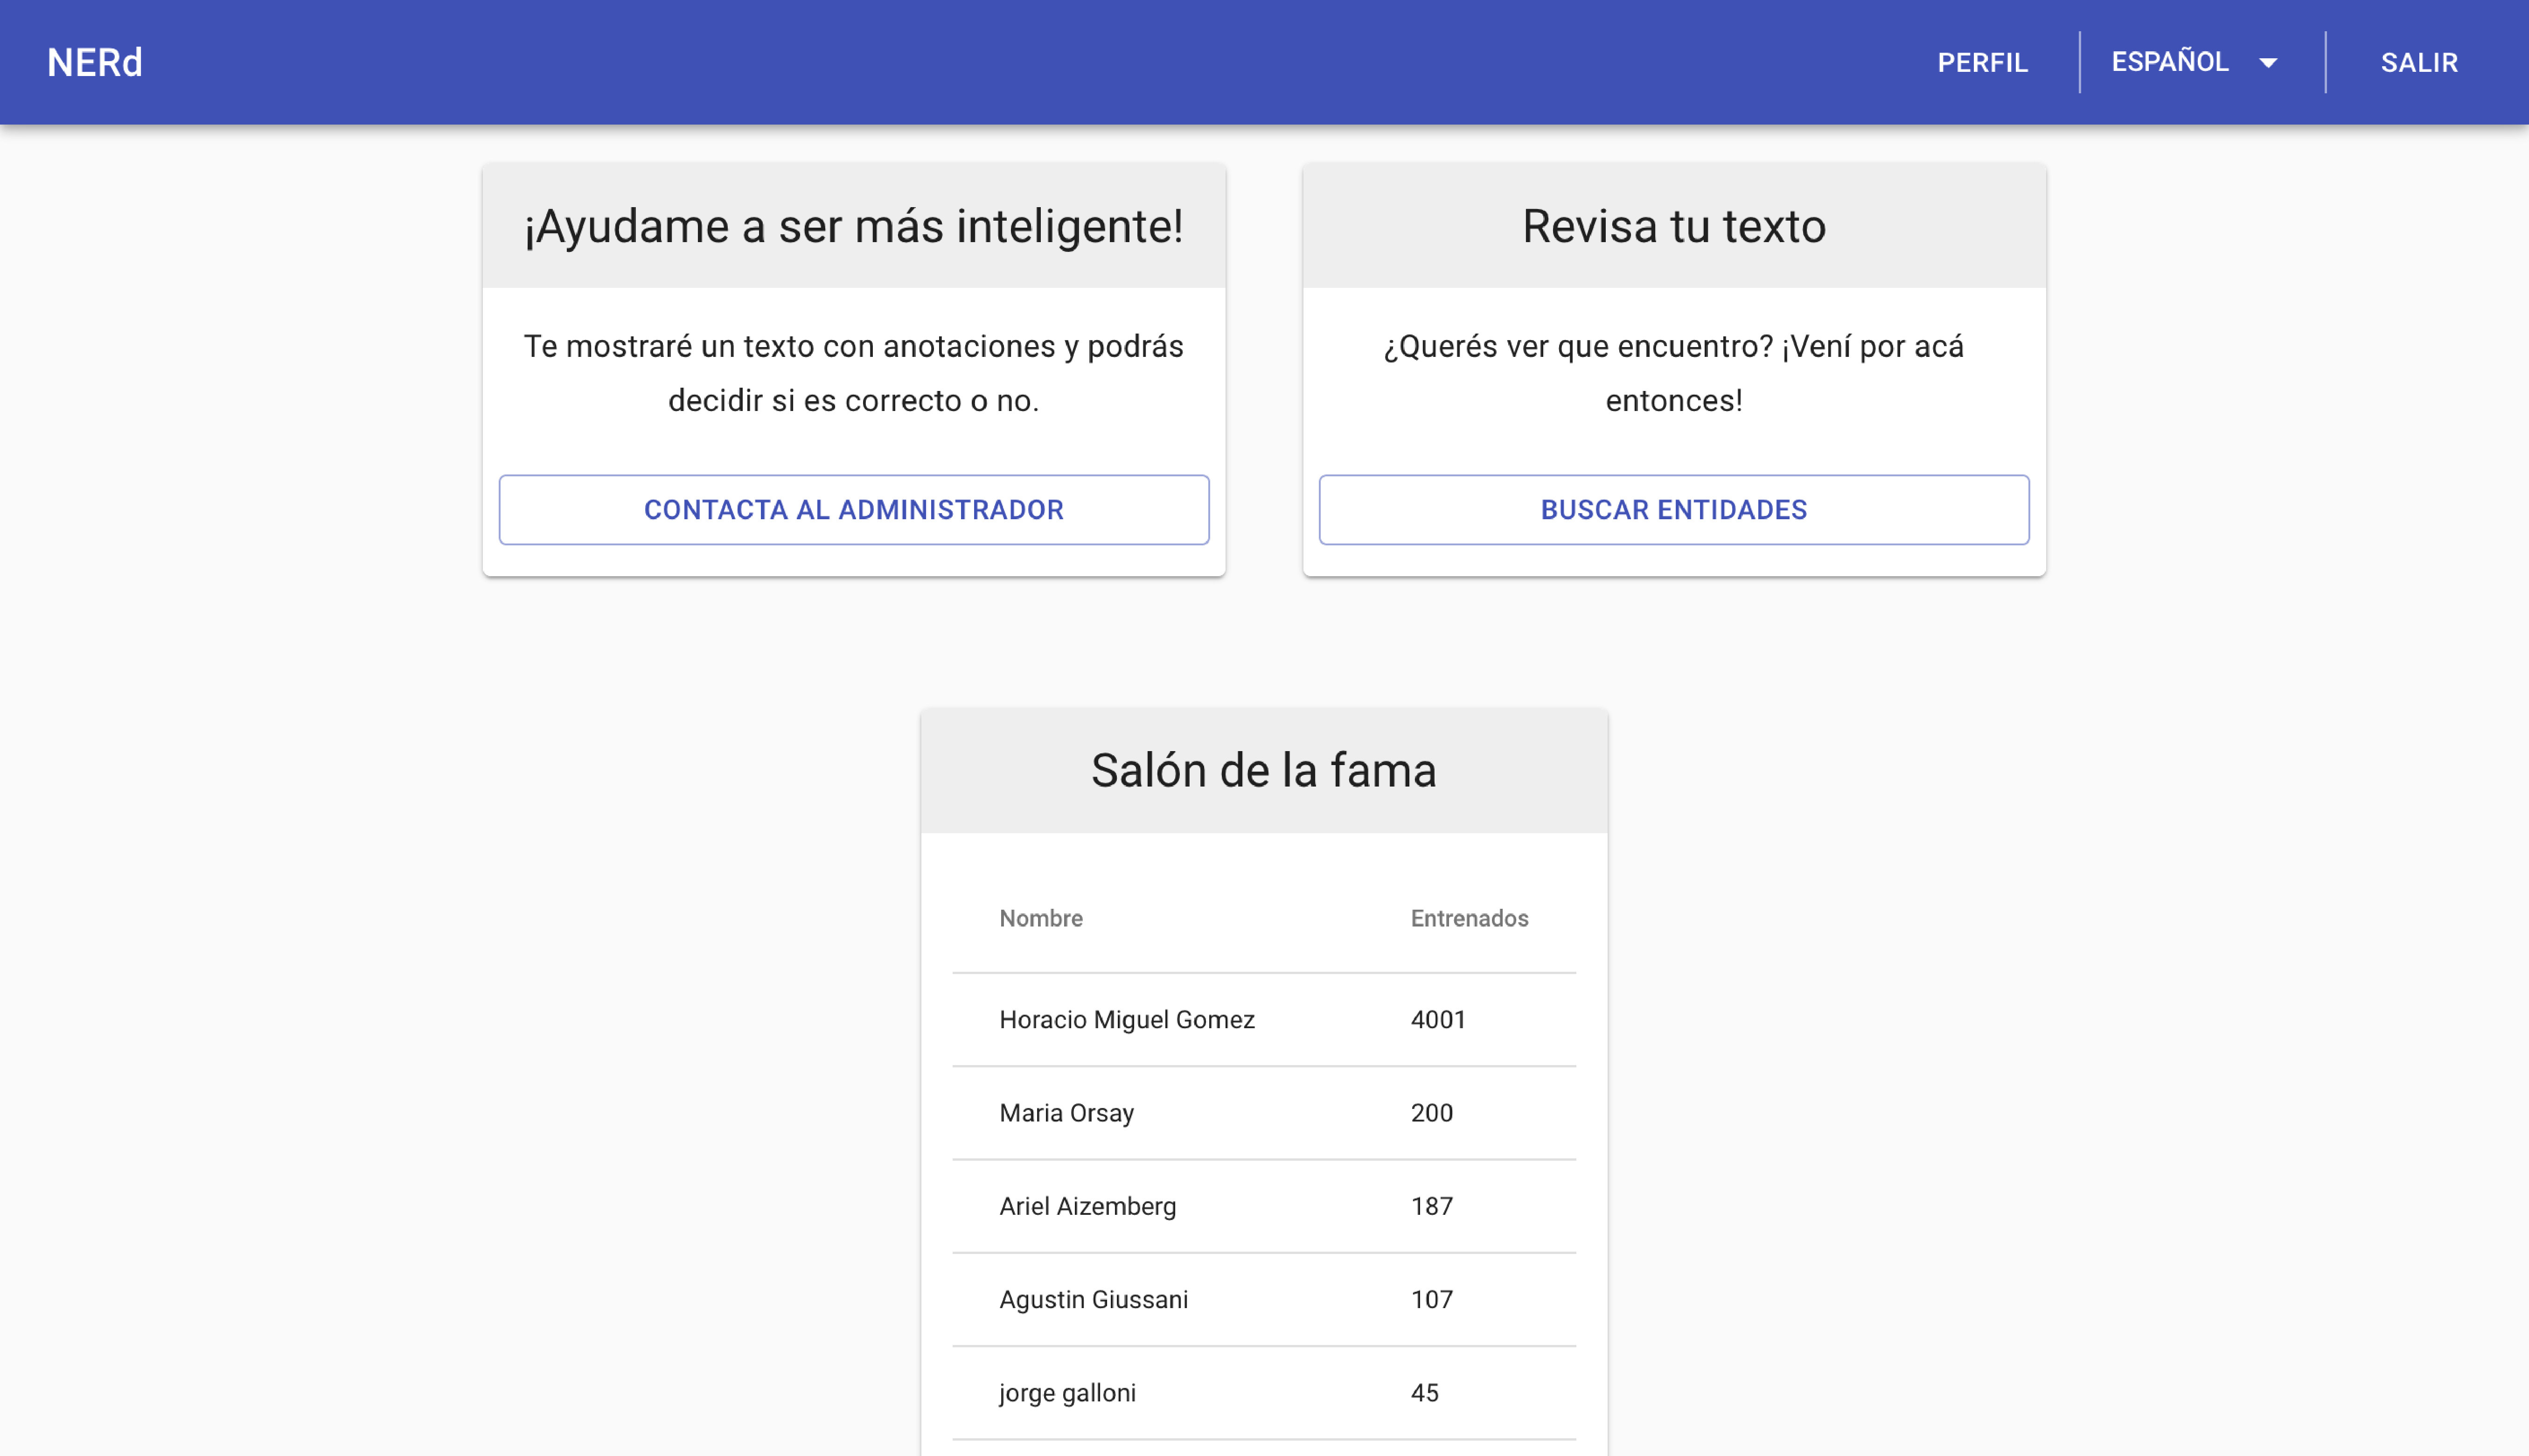
\includegraphics{assets/logic/home-logged-not_trainer.pdf} 

}

\caption{Pantalla de inicio sin rol de entrenador}\label{fig:logic-home-logged-nontrainer}
\end{figure}

Si la persona visitando la página no cuenta con una sesión activa, se le invita a ingresar con una cuenta pre-existente o a registrarse.

\begin{figure}[H]

{\centering 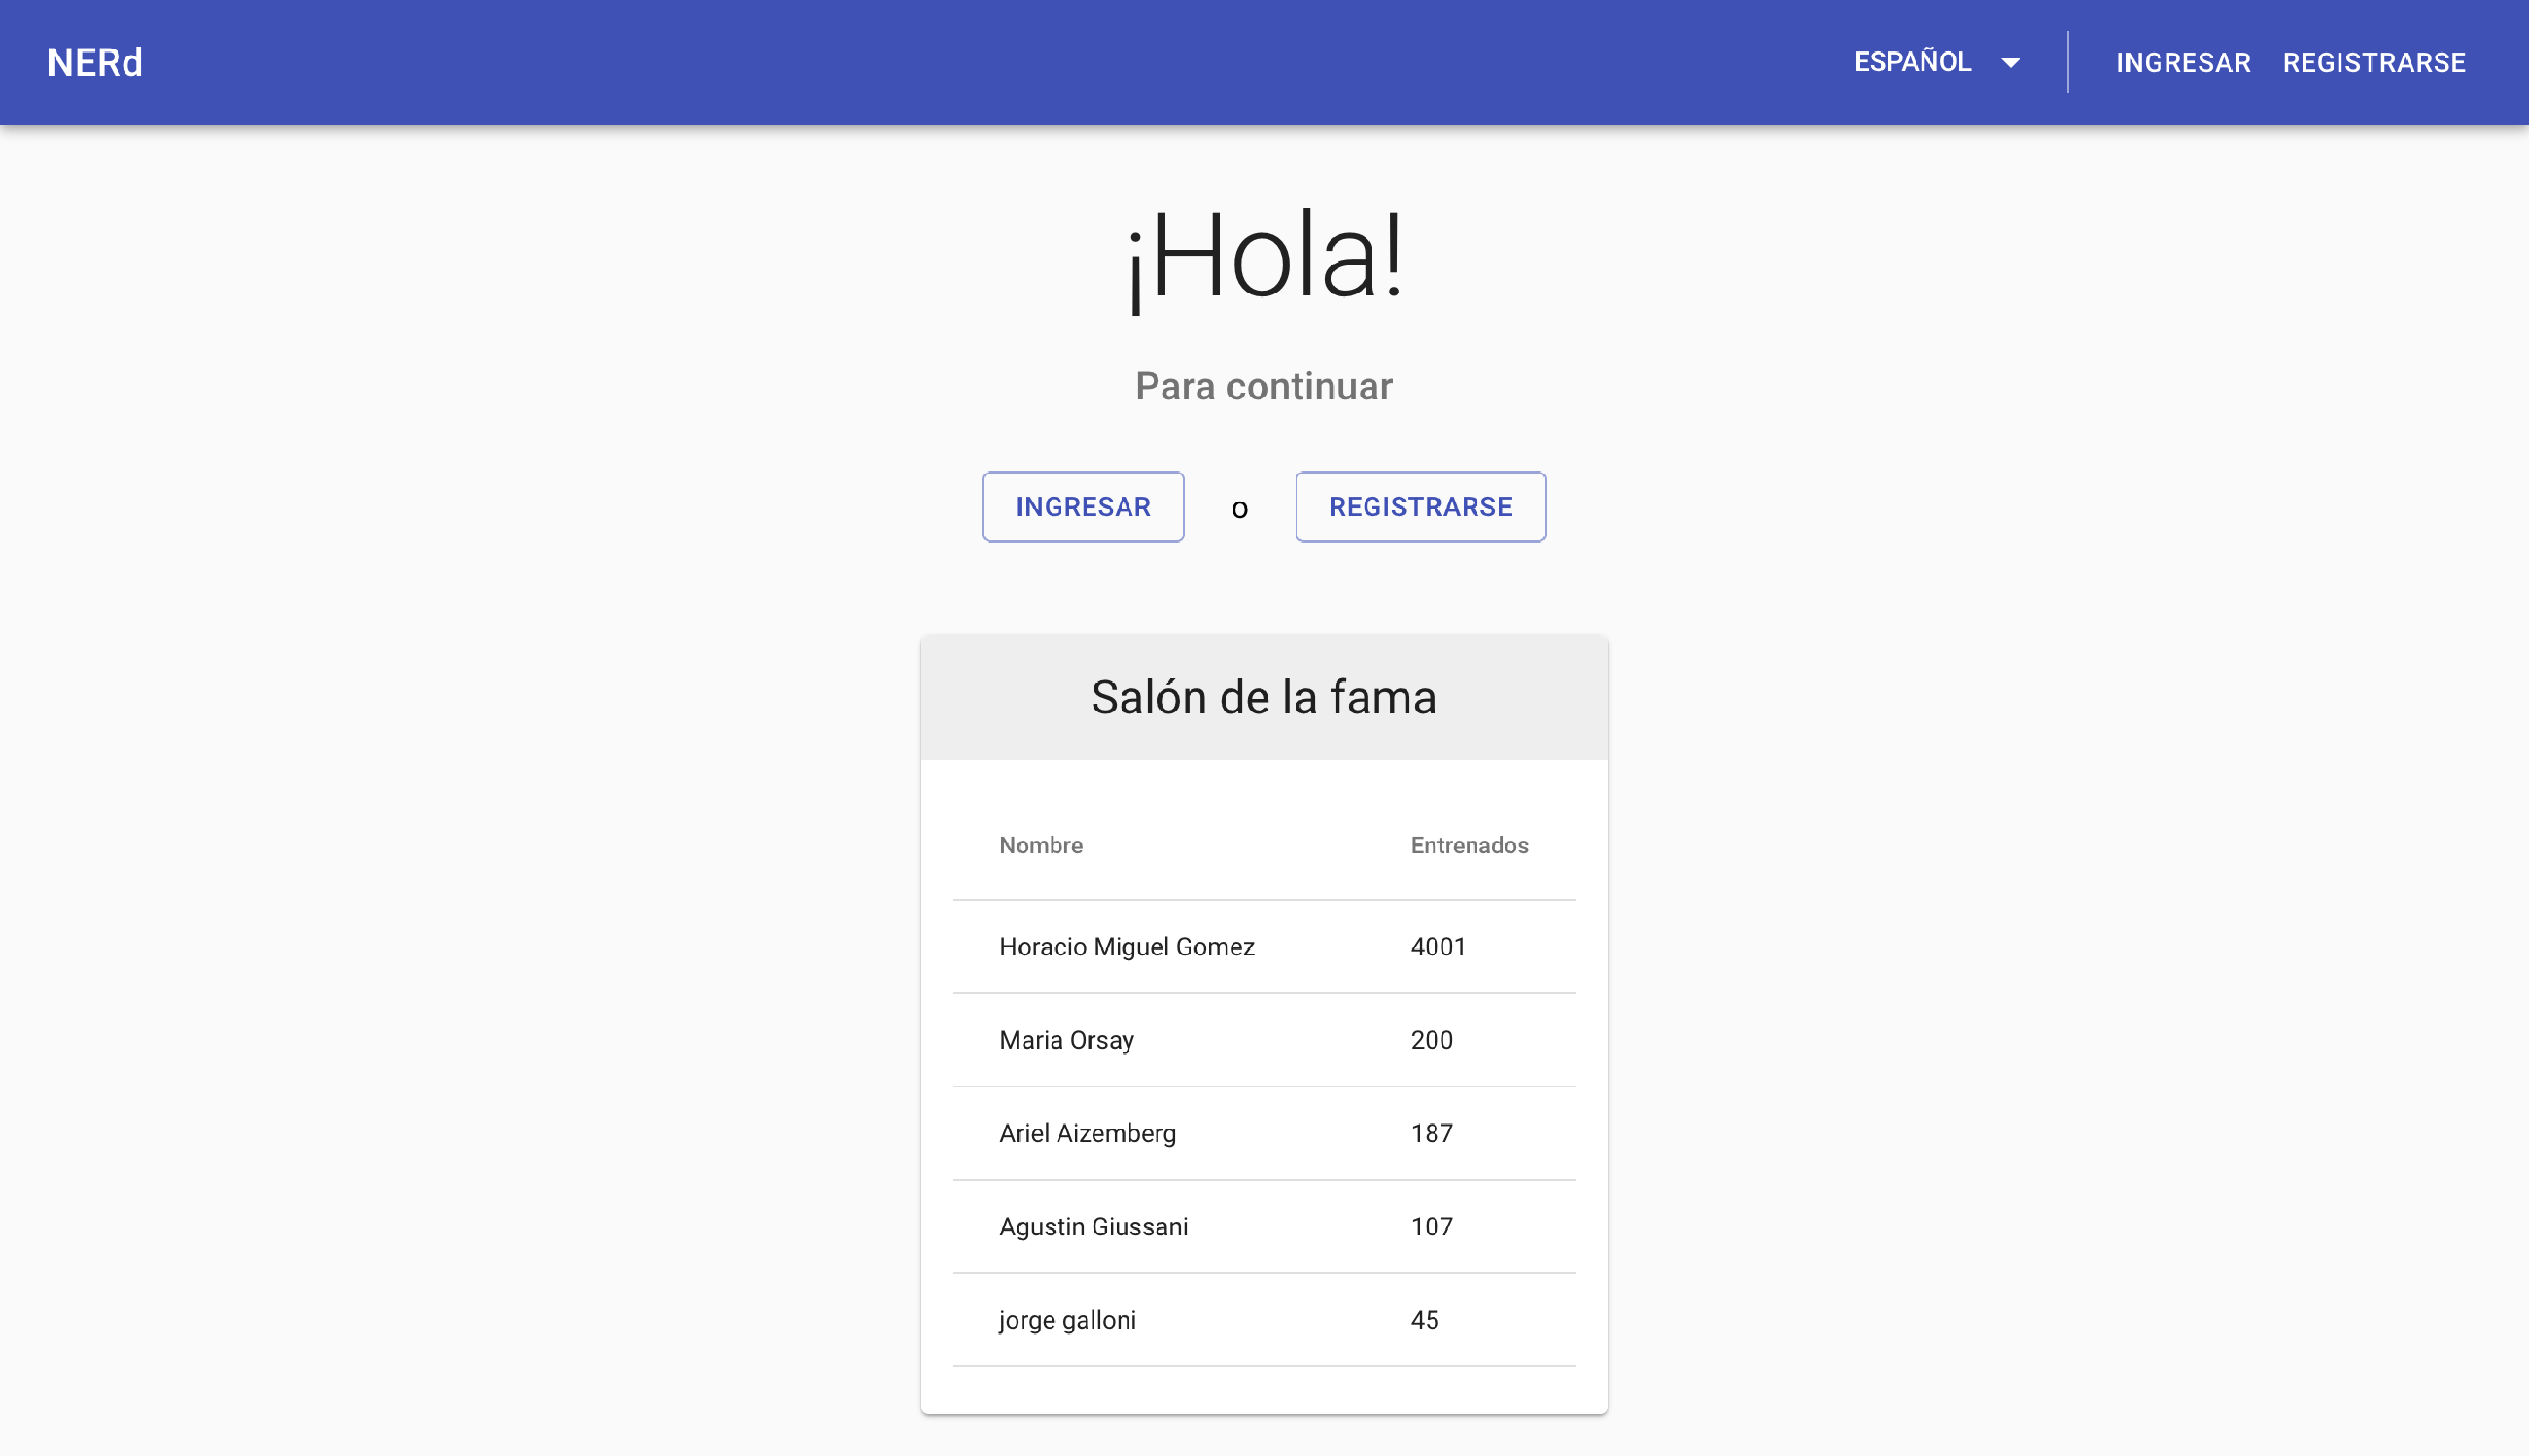
\includegraphics{assets/logic/home-anonymous.pdf} 

}

\caption{Pantalla de inicio sin sesión}\label{fig:logic-home-anonymous}
\end{figure}

\hypertarget{entrenamiento}{%
\paragraph{Entrenamiento}\label{entrenamiento}}

La pantalla de \emph{Entrenamiento} es el núcleo de la web en la cual es posible entrenar el modelo.

El usuario es presentado con un texto perteneciente al Corpus del servicio con las entidades inferidas por el modelo actual. Con un editor especial, le permitimos al usuario poder corregir las entidades inferidas y enviarle la corrección al servicio. Esa corrección será utilizada posteriormente a la hora de mejorar el modelo actual.

\begin{figure}[H]

{\centering 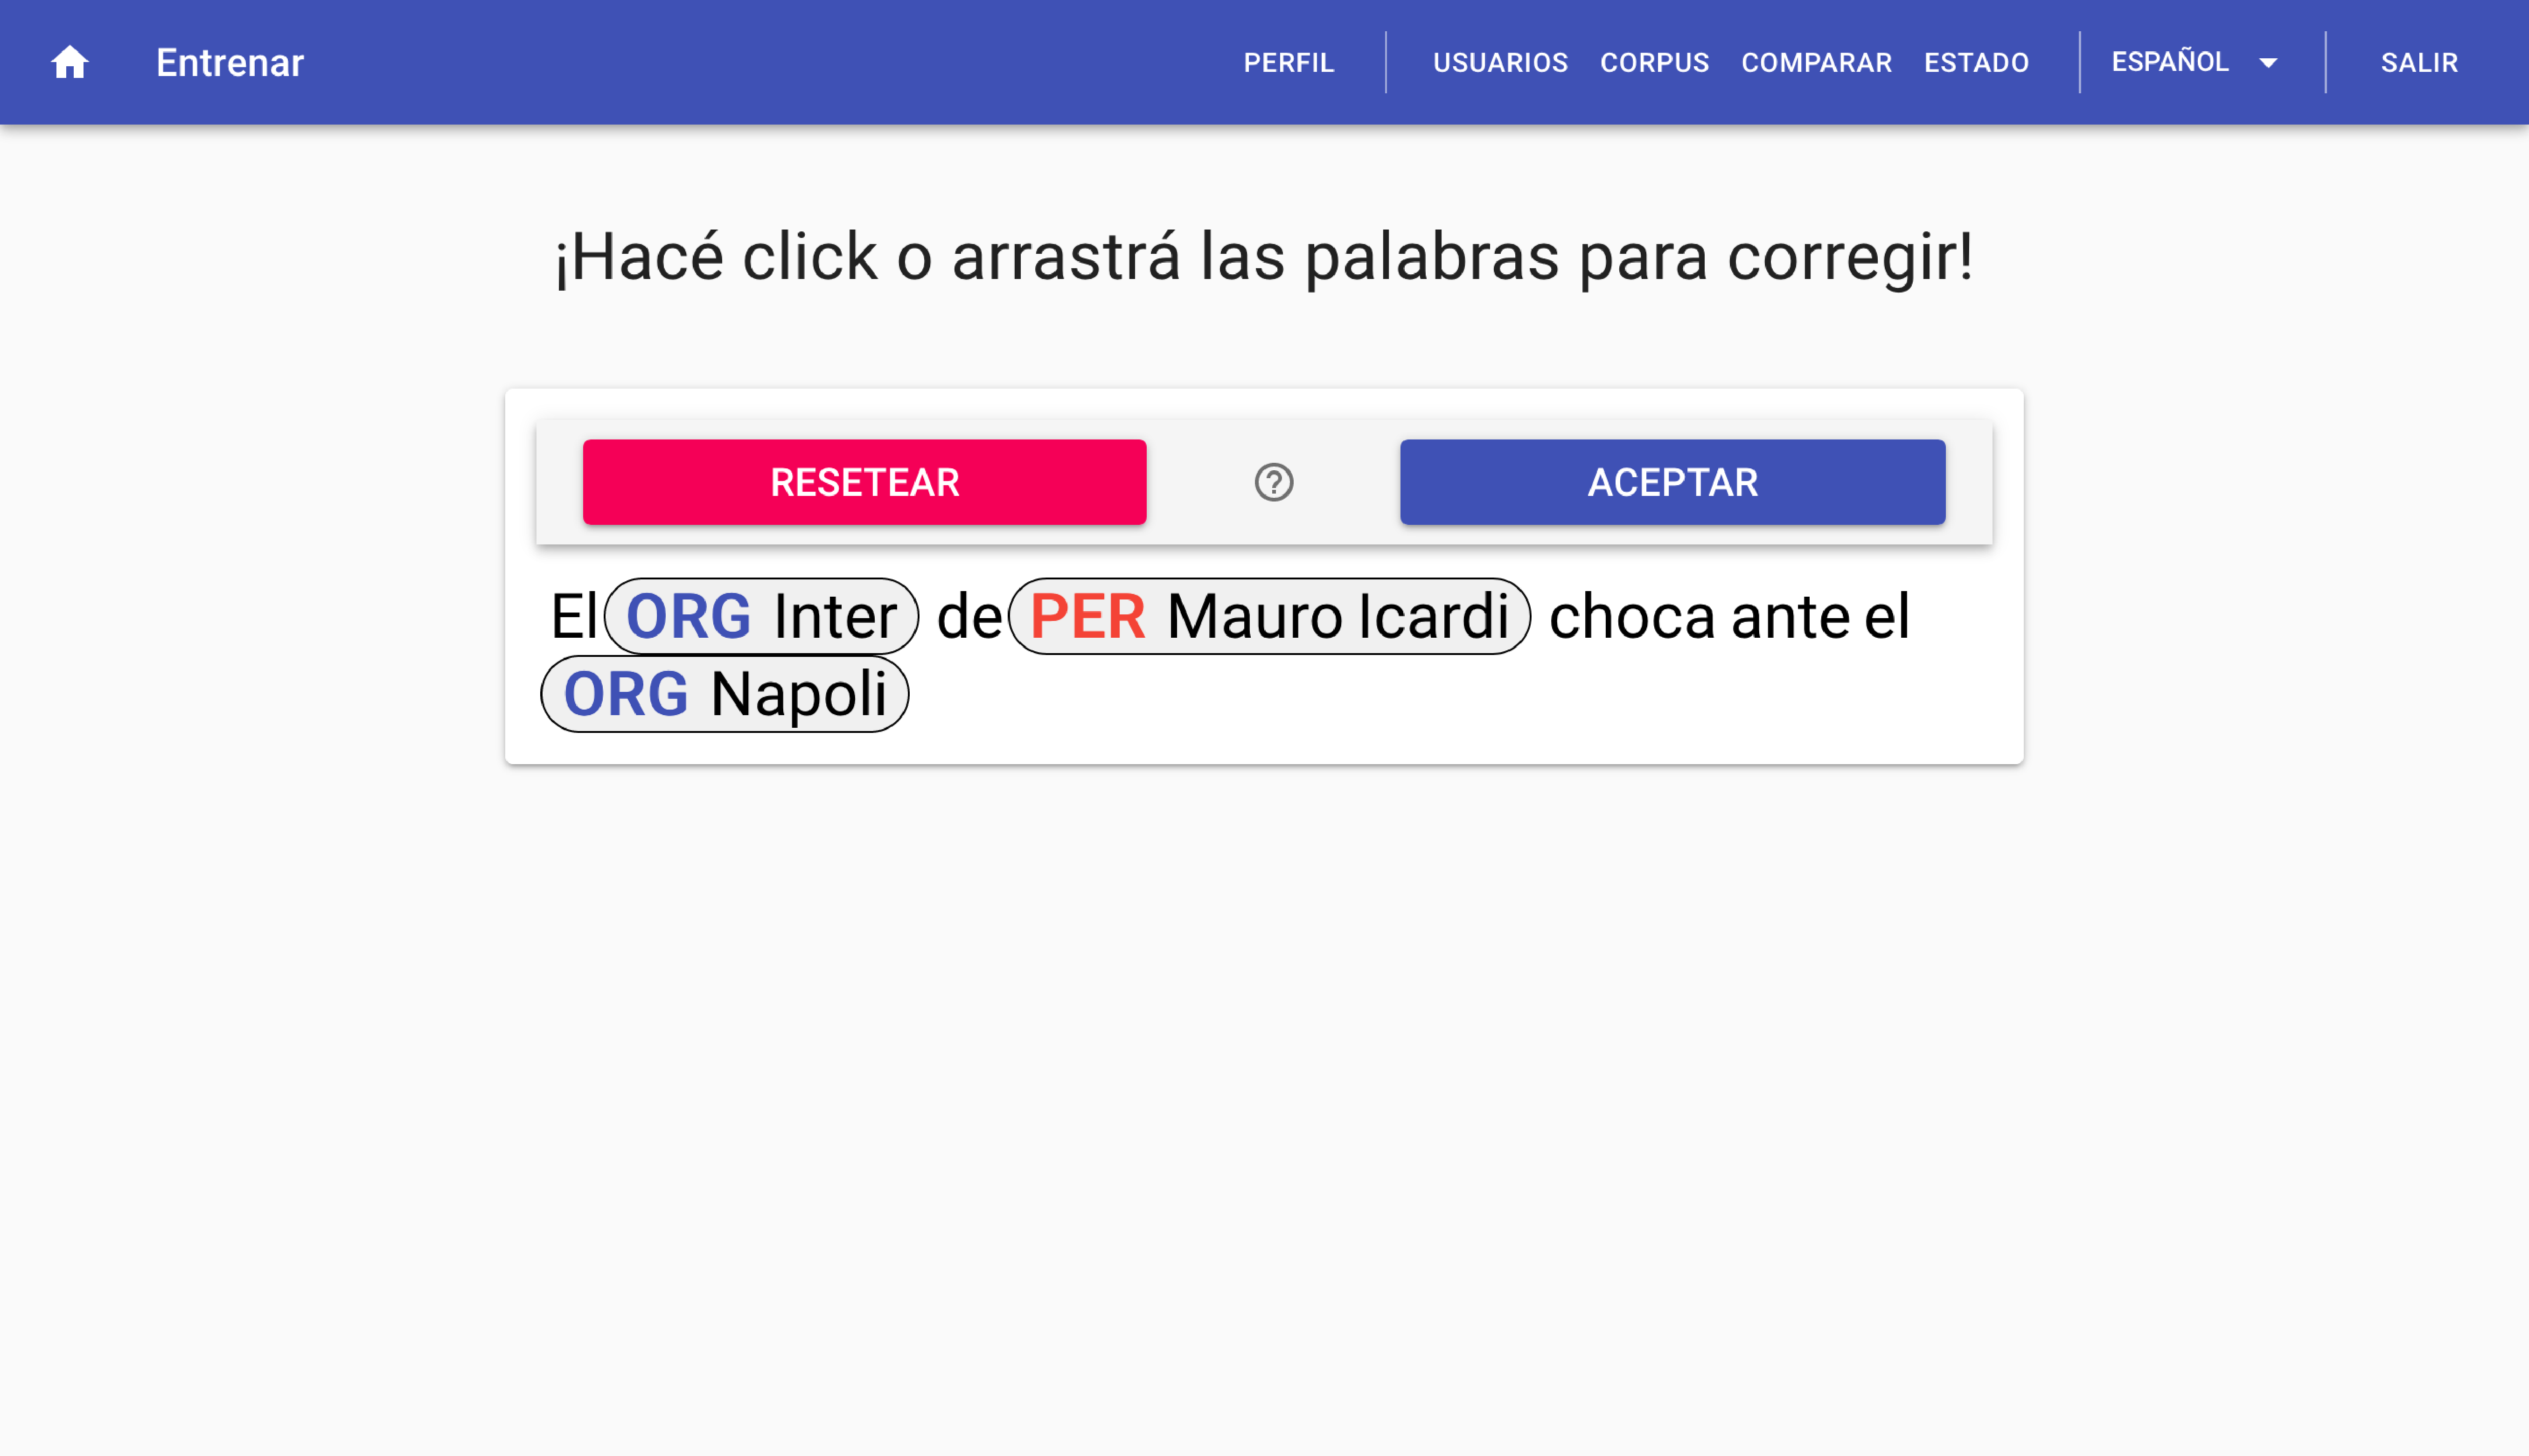
\includegraphics{assets/logic/train.pdf} 

}

\caption{Pantalla de entrenamiento}\label{fig:logic-train}
\end{figure}

\hypertarget{usabilidad}{%
\subparagraph{Usabilidad}\label{usabilidad}}

Tuvimos un foco fuerte en la usabilidad del widget ya que los entrenadores del servicio van a pasar prácticamente todo su tiempo en ésta pantalla, por lo que se tuvieron las siguientes consideraciones en la implementación.

Llamado a acción y ayuda

Dado que lo primero que ve el usuario es un texto con anotaciones, agregamos un título que invita al usuario a realizar acciones sobre el texto. De esta manera, le mostramos las dos acciones principales realizables desde el widget de entrenamiento: Click en alguna palabra o entidad y arrastrar un conjunto de palabras para crear una entidad nueva.
Como refuerzo de este llamado a acción, agregamos un botón que al ser clickeado muestra un mensaje de ayuda con instrucciones más detalladas sobre el objetivo del entrenador y las acciones que deben de realizarse sobre el mismo.

\begin{figure}[H]

{\centering 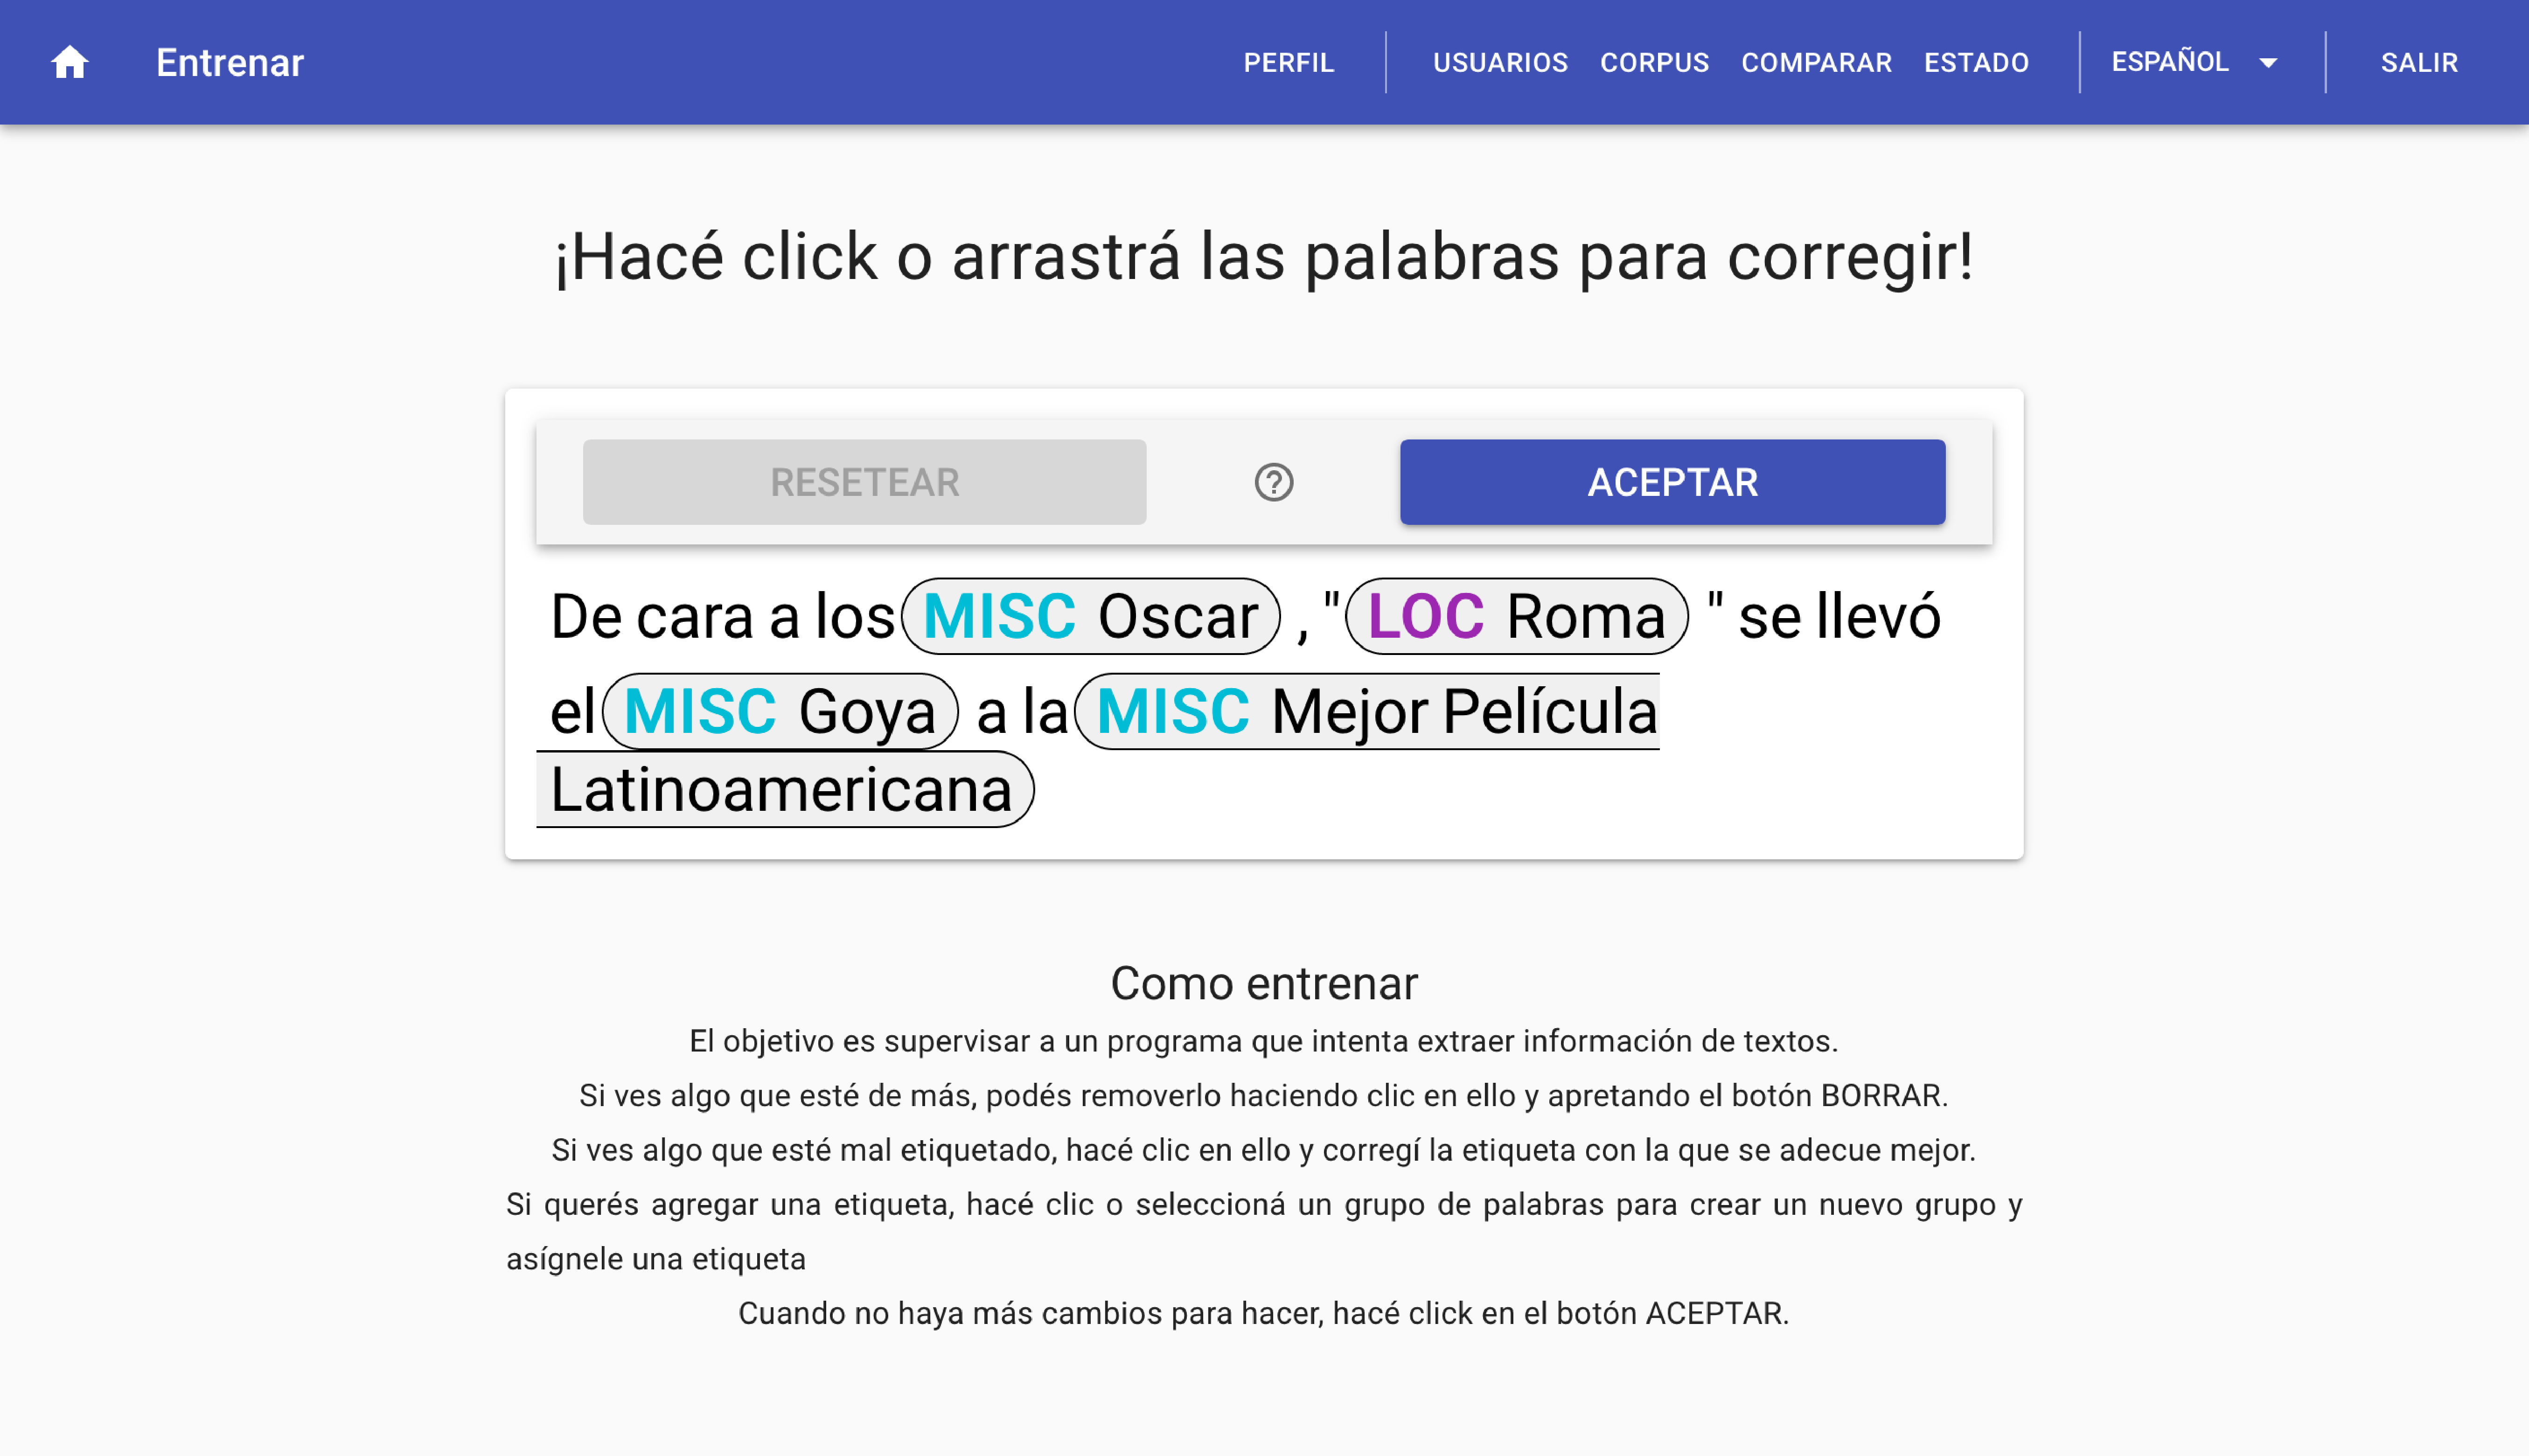
\includegraphics{assets/logic/train-help.pdf} 

}

\caption{Ayuda del entrenador}\label{fig:logic-train-help}
\end{figure}

Creación y edición de entidades

Para la creación de entidades decidimos ofrecer dos maneras: La primera es arrastrando un conjunto de palabras de manera tal de unirlas todas en una única entidad.
La otra es hacer click en una palabra y ahí se ofrecen opciones dependiendo de la ubicación de la palabra dentro del texto:

\begin{itemize}
\tightlist
\item
  Si no existen entidades en el texto actual, se le asigna por defecto el tipo \emph{MISC} y se muestran el resto de los tipos para permitir cambiarlo de ser necesario.
\item
  Si existen entidades antes o después, se ofrece la opción de unir la palabra actual con la entidada más próxima para el lado elegido.
\end{itemize}

\begin{figure}[H]

{\centering 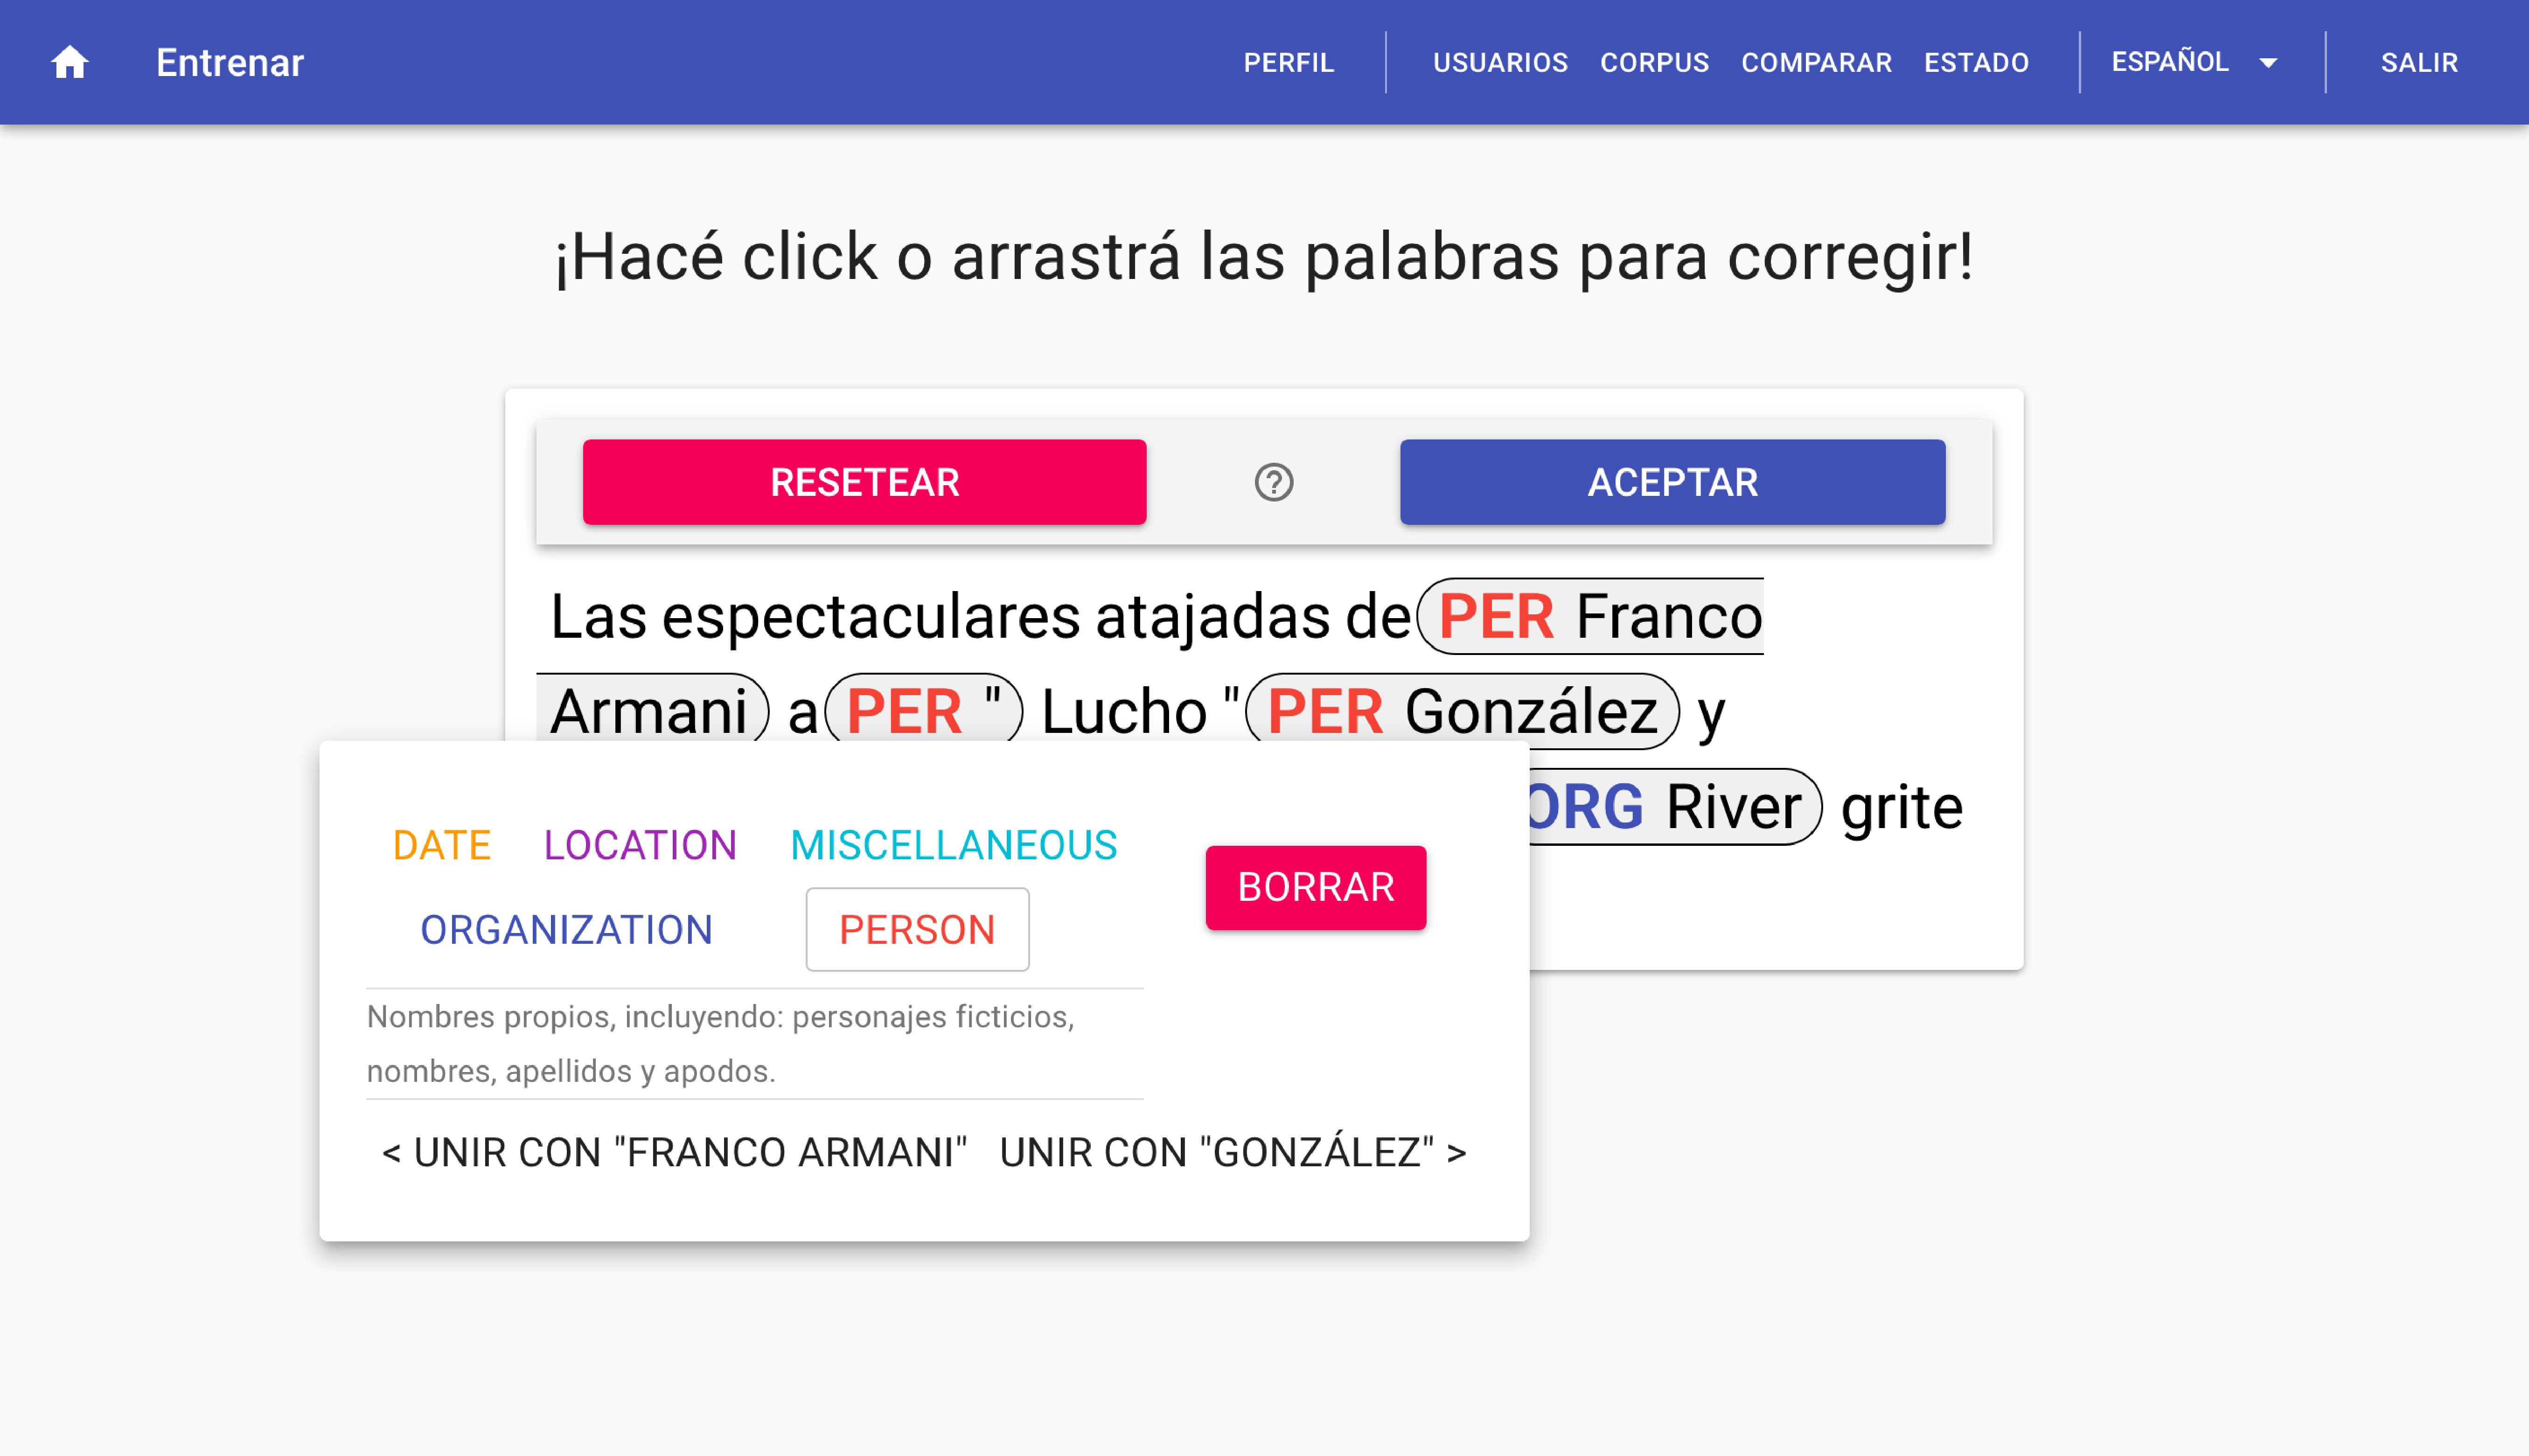
\includegraphics{assets/logic/train-popup.pdf} 

}

\caption{Edición de entidad}\label{fig:logic-train-popup}
\end{figure}

Para la edición de entidades decidimos permitir únicamente la modificación del tipo de una entidad inferida.
Si el modelo infirió una entidad de manera incorrecta, ya sea por que sea una entidad inválida o agregó palabras de más a una entidad inválida, permitimos que el usuario remueva la entidad y que después vuelva a agregar la entidad correcta.

Optimización en tiempos de carga

Dado que es esperado que un usuario entrene más de un texto, al momento de pedir un texto para mostrar, se pide el siguiente. Mediante este mecanismo de pre-carga, podemos eliminar el tiempo de espera entre texto y texto ofreciendo al usuario una experiencia completamente fluida.

\hypertarget{administraciuxf3n-de-usuarios}{%
\paragraph{Administración de usuarios}\label{administraciuxf3n-de-usuarios}}

La pantalla de \emph{Administración de usuarios} permite a los usuarios con el rol de administrador poder modificar los roles de todos los usuarios del sistema, borrarlos o acceder a los detalles del usuario, tal como la lista de textos entrenados.

\begin{figure}[H]

{\centering 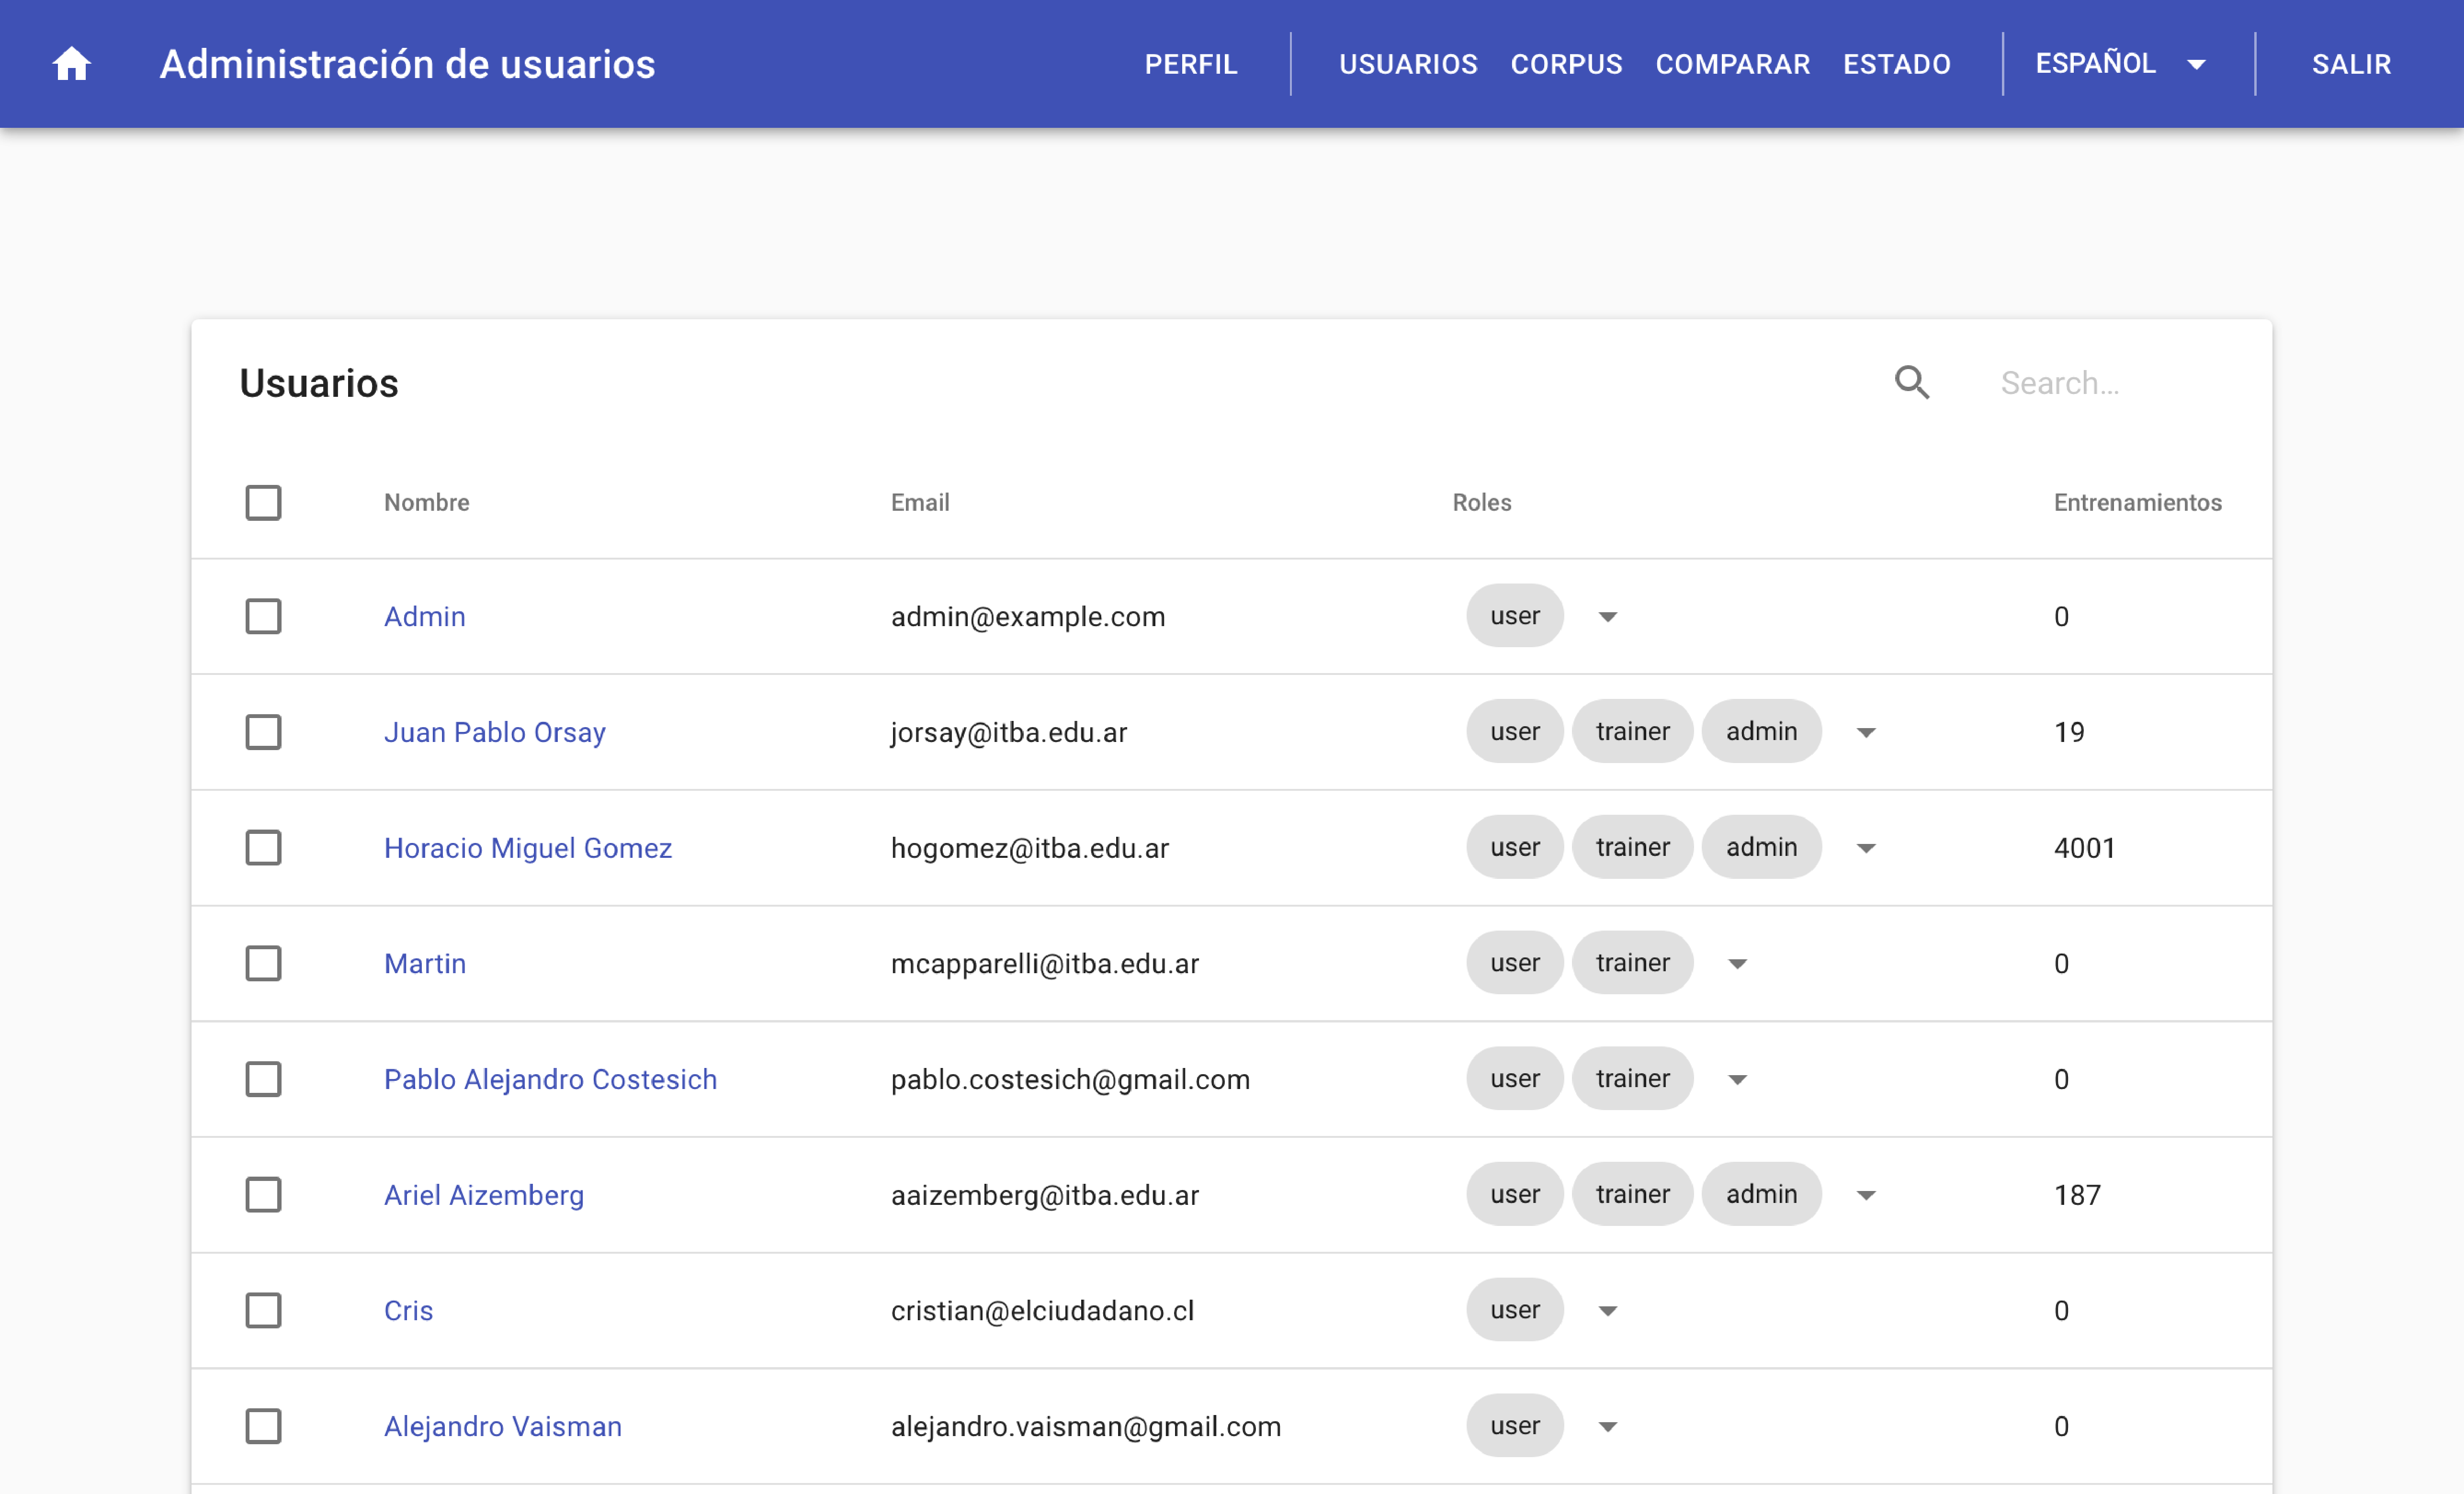
\includegraphics{assets/logic/user-list.pdf} 

}

\caption{Administración de usuarios}\label{fig:logic-user-list}
\end{figure}

\hypertarget{detalles-de-usuario}{%
\paragraph{Detalles de usuario}\label{detalles-de-usuario}}

La pantalla de detalle de usuario permite al usuario con sesión activa ver sus entrenamientos y cambiar su contraseña.

Los usuarios con rol administrador pueden realizar las acciones mencionadas previamente pero a otros usuarios.

\begin{figure}[H]

{\centering 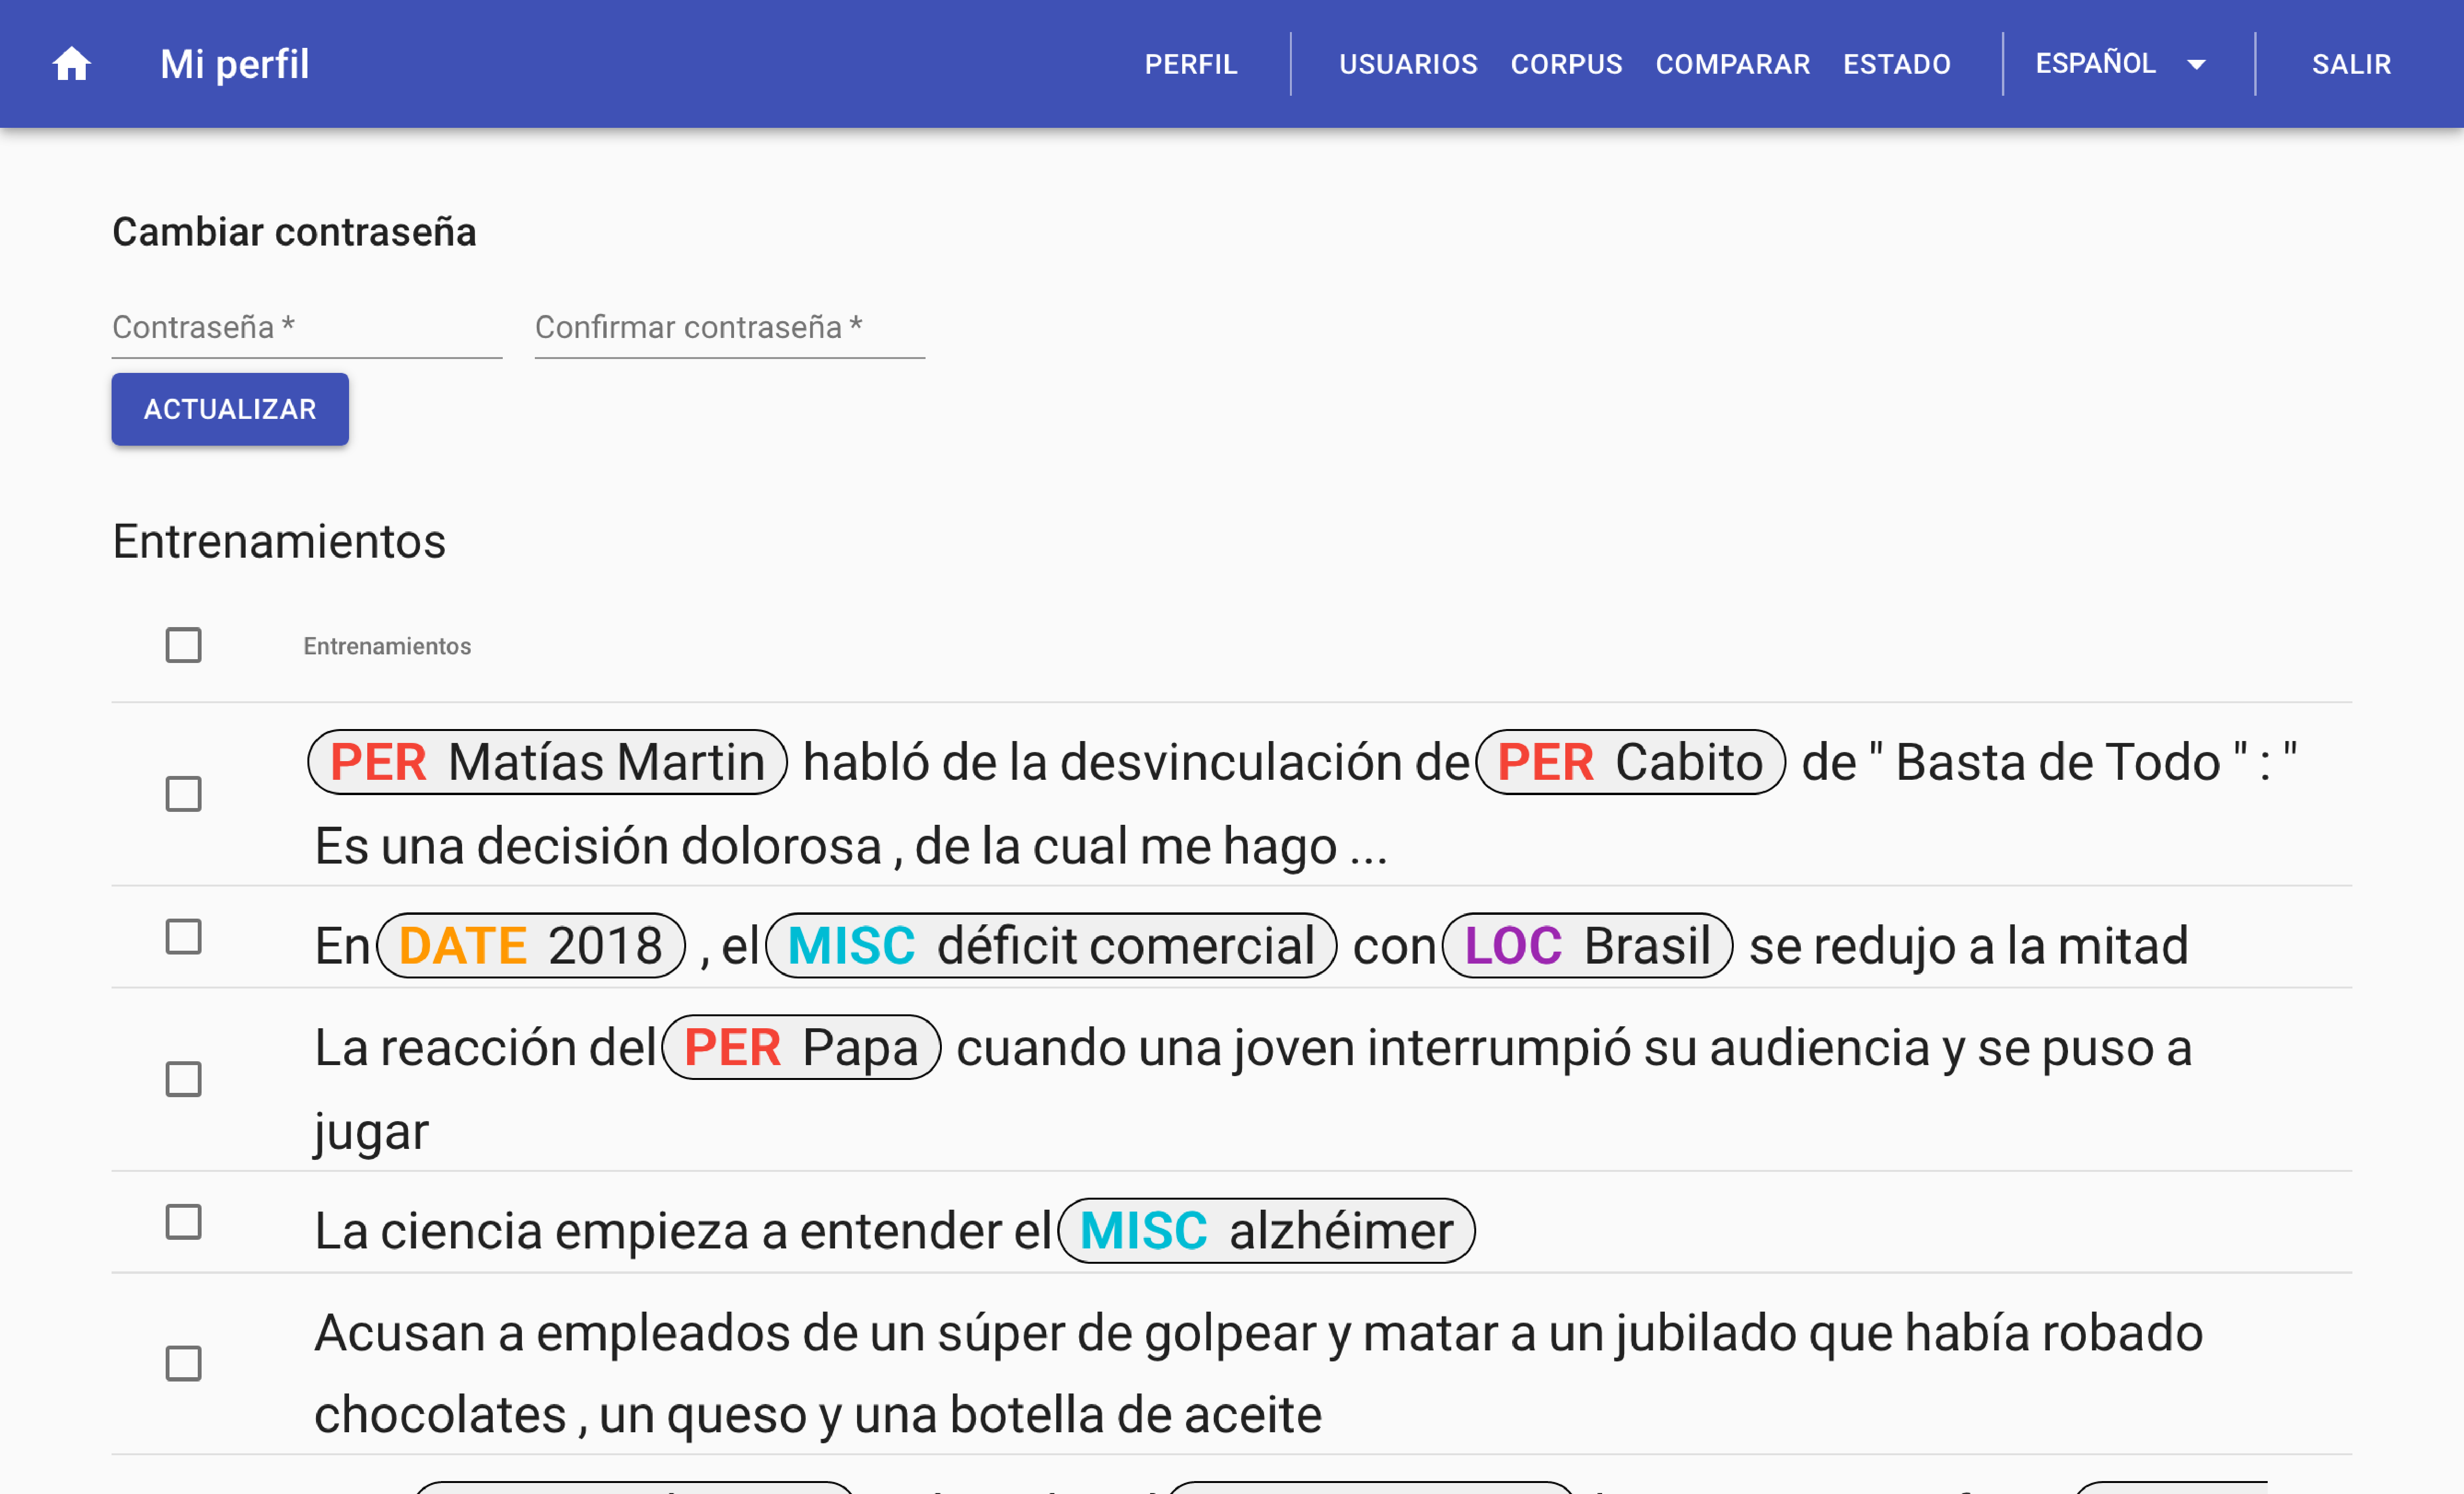
\includegraphics{assets/logic/user-profile.pdf} 

}

\caption{Perfil de usuario}\label{fig:logic-user-profile}
\end{figure}

\hypertarget{corpus-1}{%
\paragraph{Corpus}\label{corpus-1}}

La pantalla de \emph{Corpus} permite a un usuario con el rol de administrador realizar tareas relacionadas con el corpus del sistema.

\begin{figure}[H]

{\centering 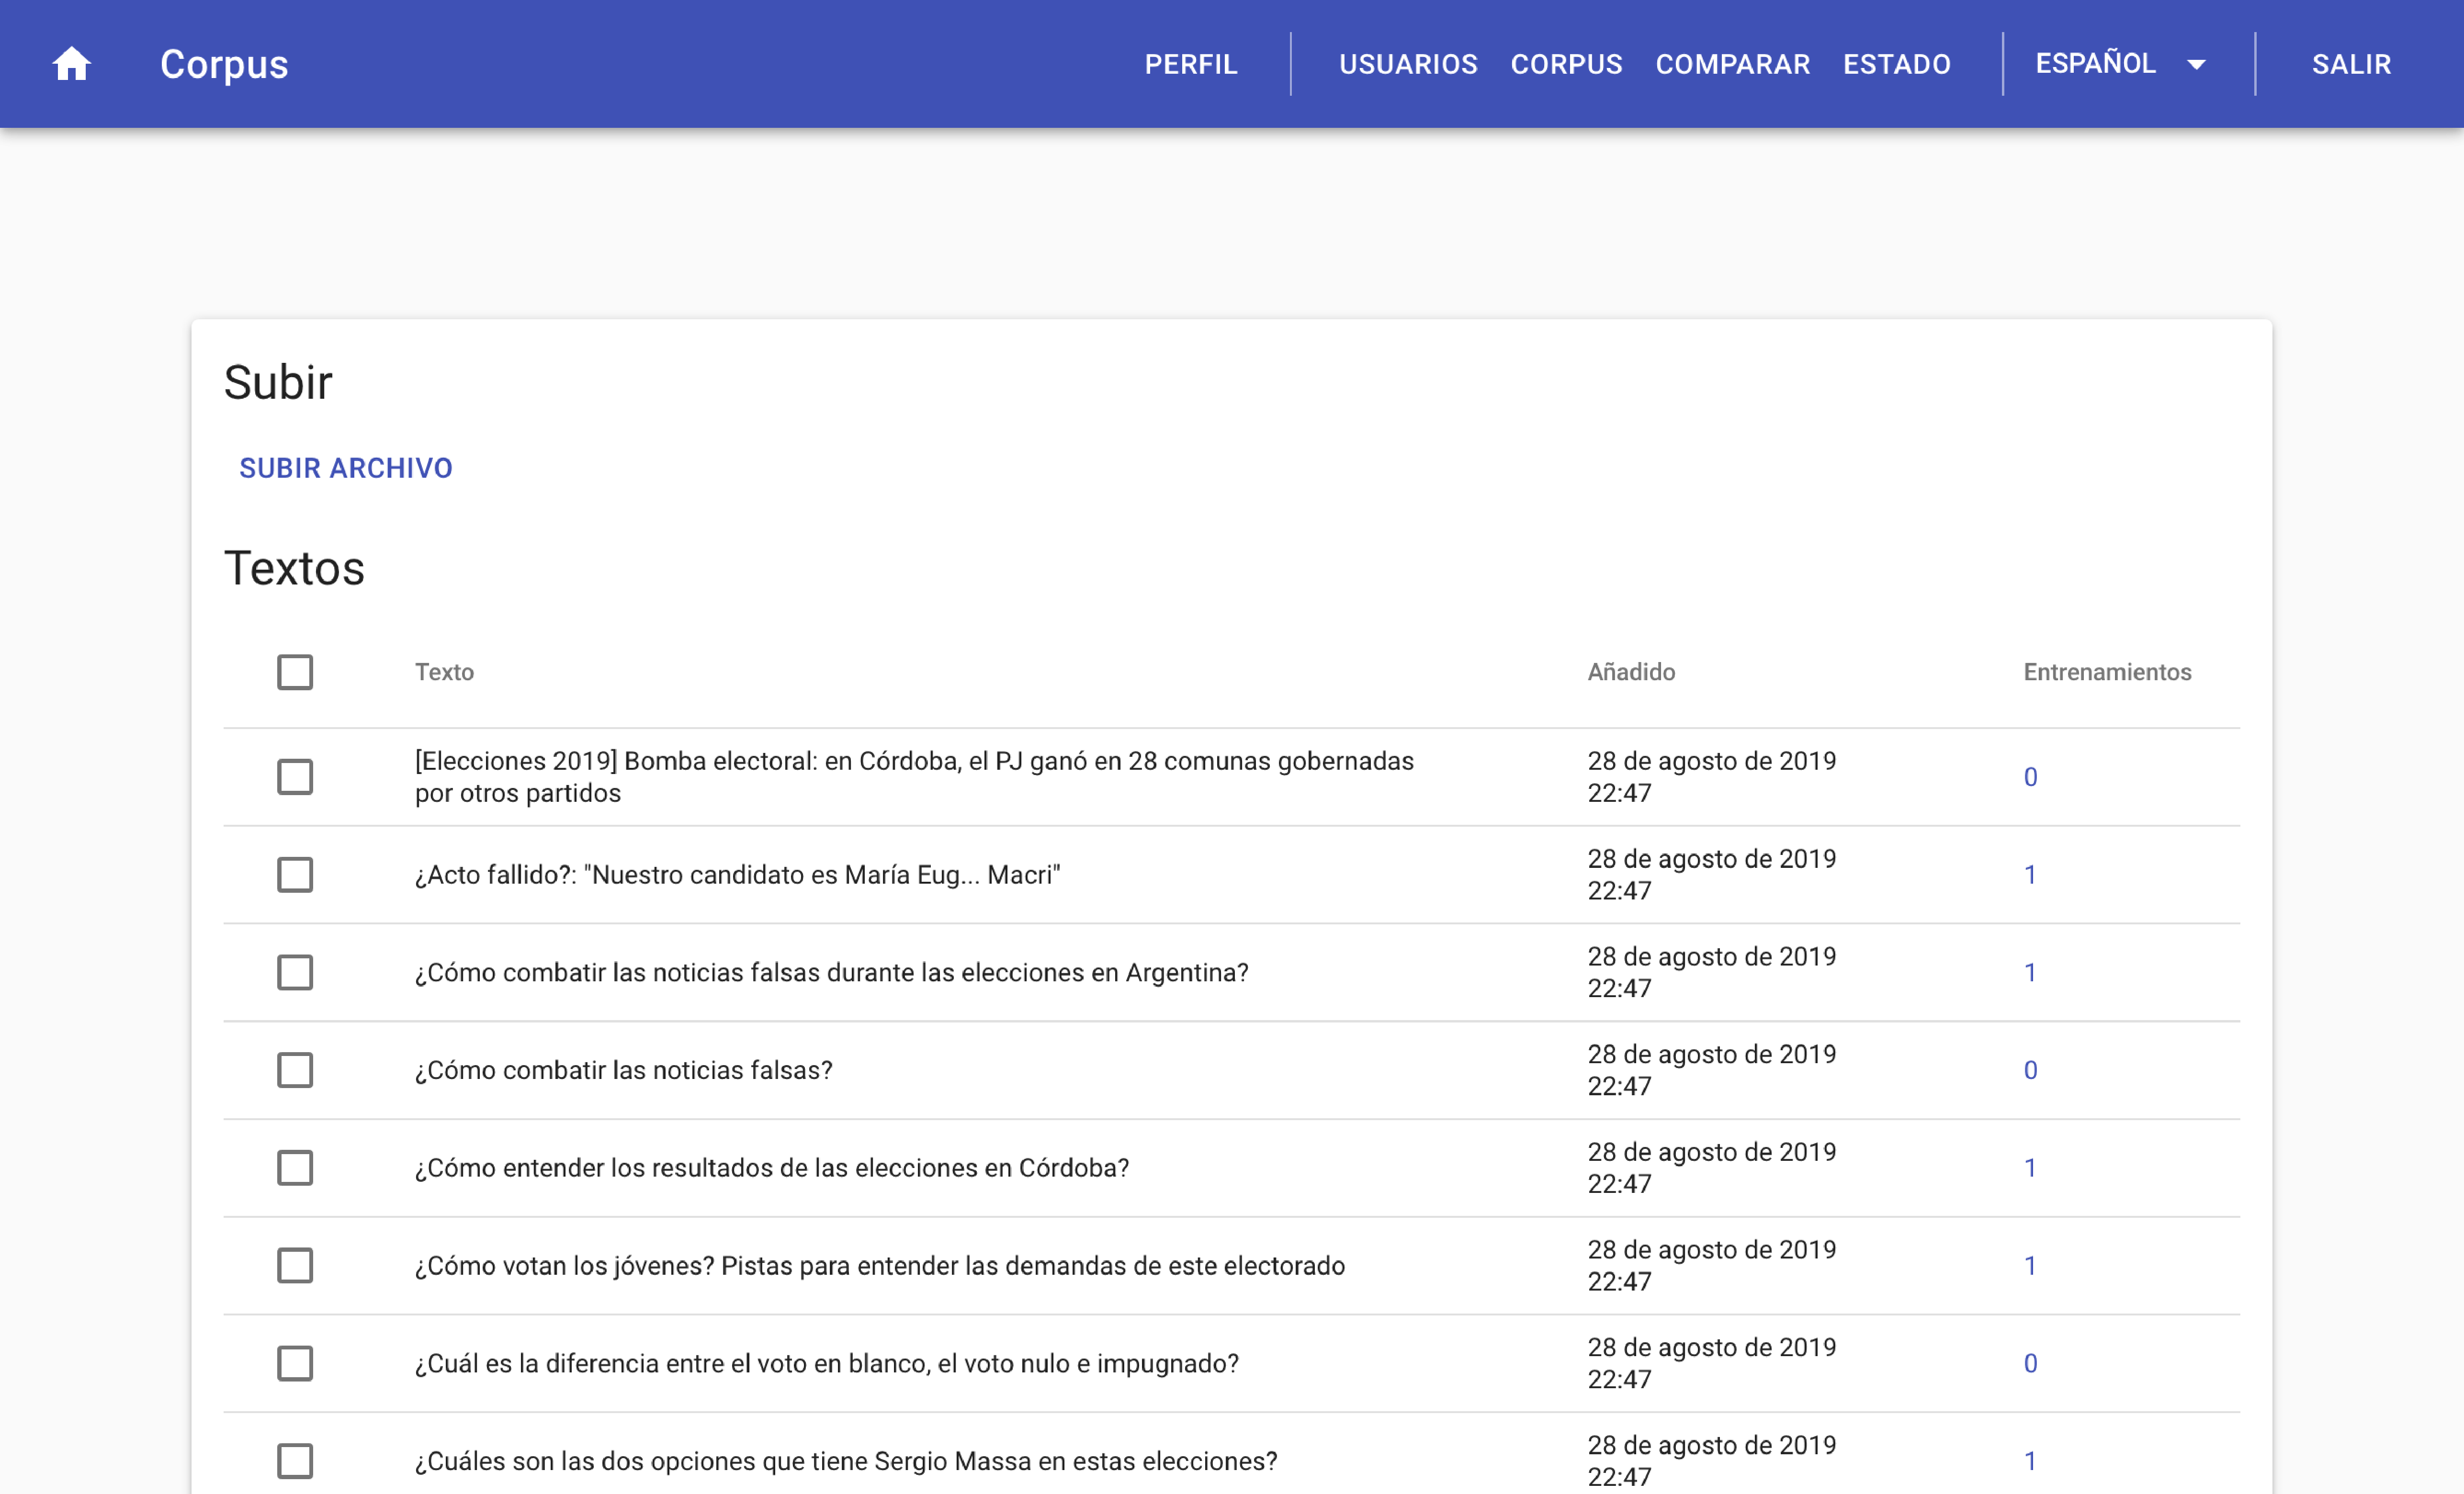
\includegraphics{assets/logic/corpus-management.pdf} 

}

\caption{Administración de corpus}\label{fig:logic-corpus-management}
\end{figure}

Desde aquí es posible agregar textos al corpus utilizando la funcionalidad de subida de archivos. Los archivos deben ser archivos con extensión \emph{.txt} y cada línea del archivo será agregada al corpus como un texto individual.

También es posible desde aquí ver todos los textos que forman parte del corpus así como también poder ver los entrenamientos para cada uno de los textos. Finalmente, es posible quitar textos del corpus así como también es posible eliminar correcciones a las inferencias de entidades cargados por usuarios.

\hypertarget{estado}{%
\paragraph{Estado}\label{estado}}

La pantalla de \emph{Estado} permite a un usuario con el rol de administrador visualizar el estado de entrenamiento del corpus así como también realizar diversas acciones sobre los \emph{workers}.

\begin{figure}[H]

{\centering 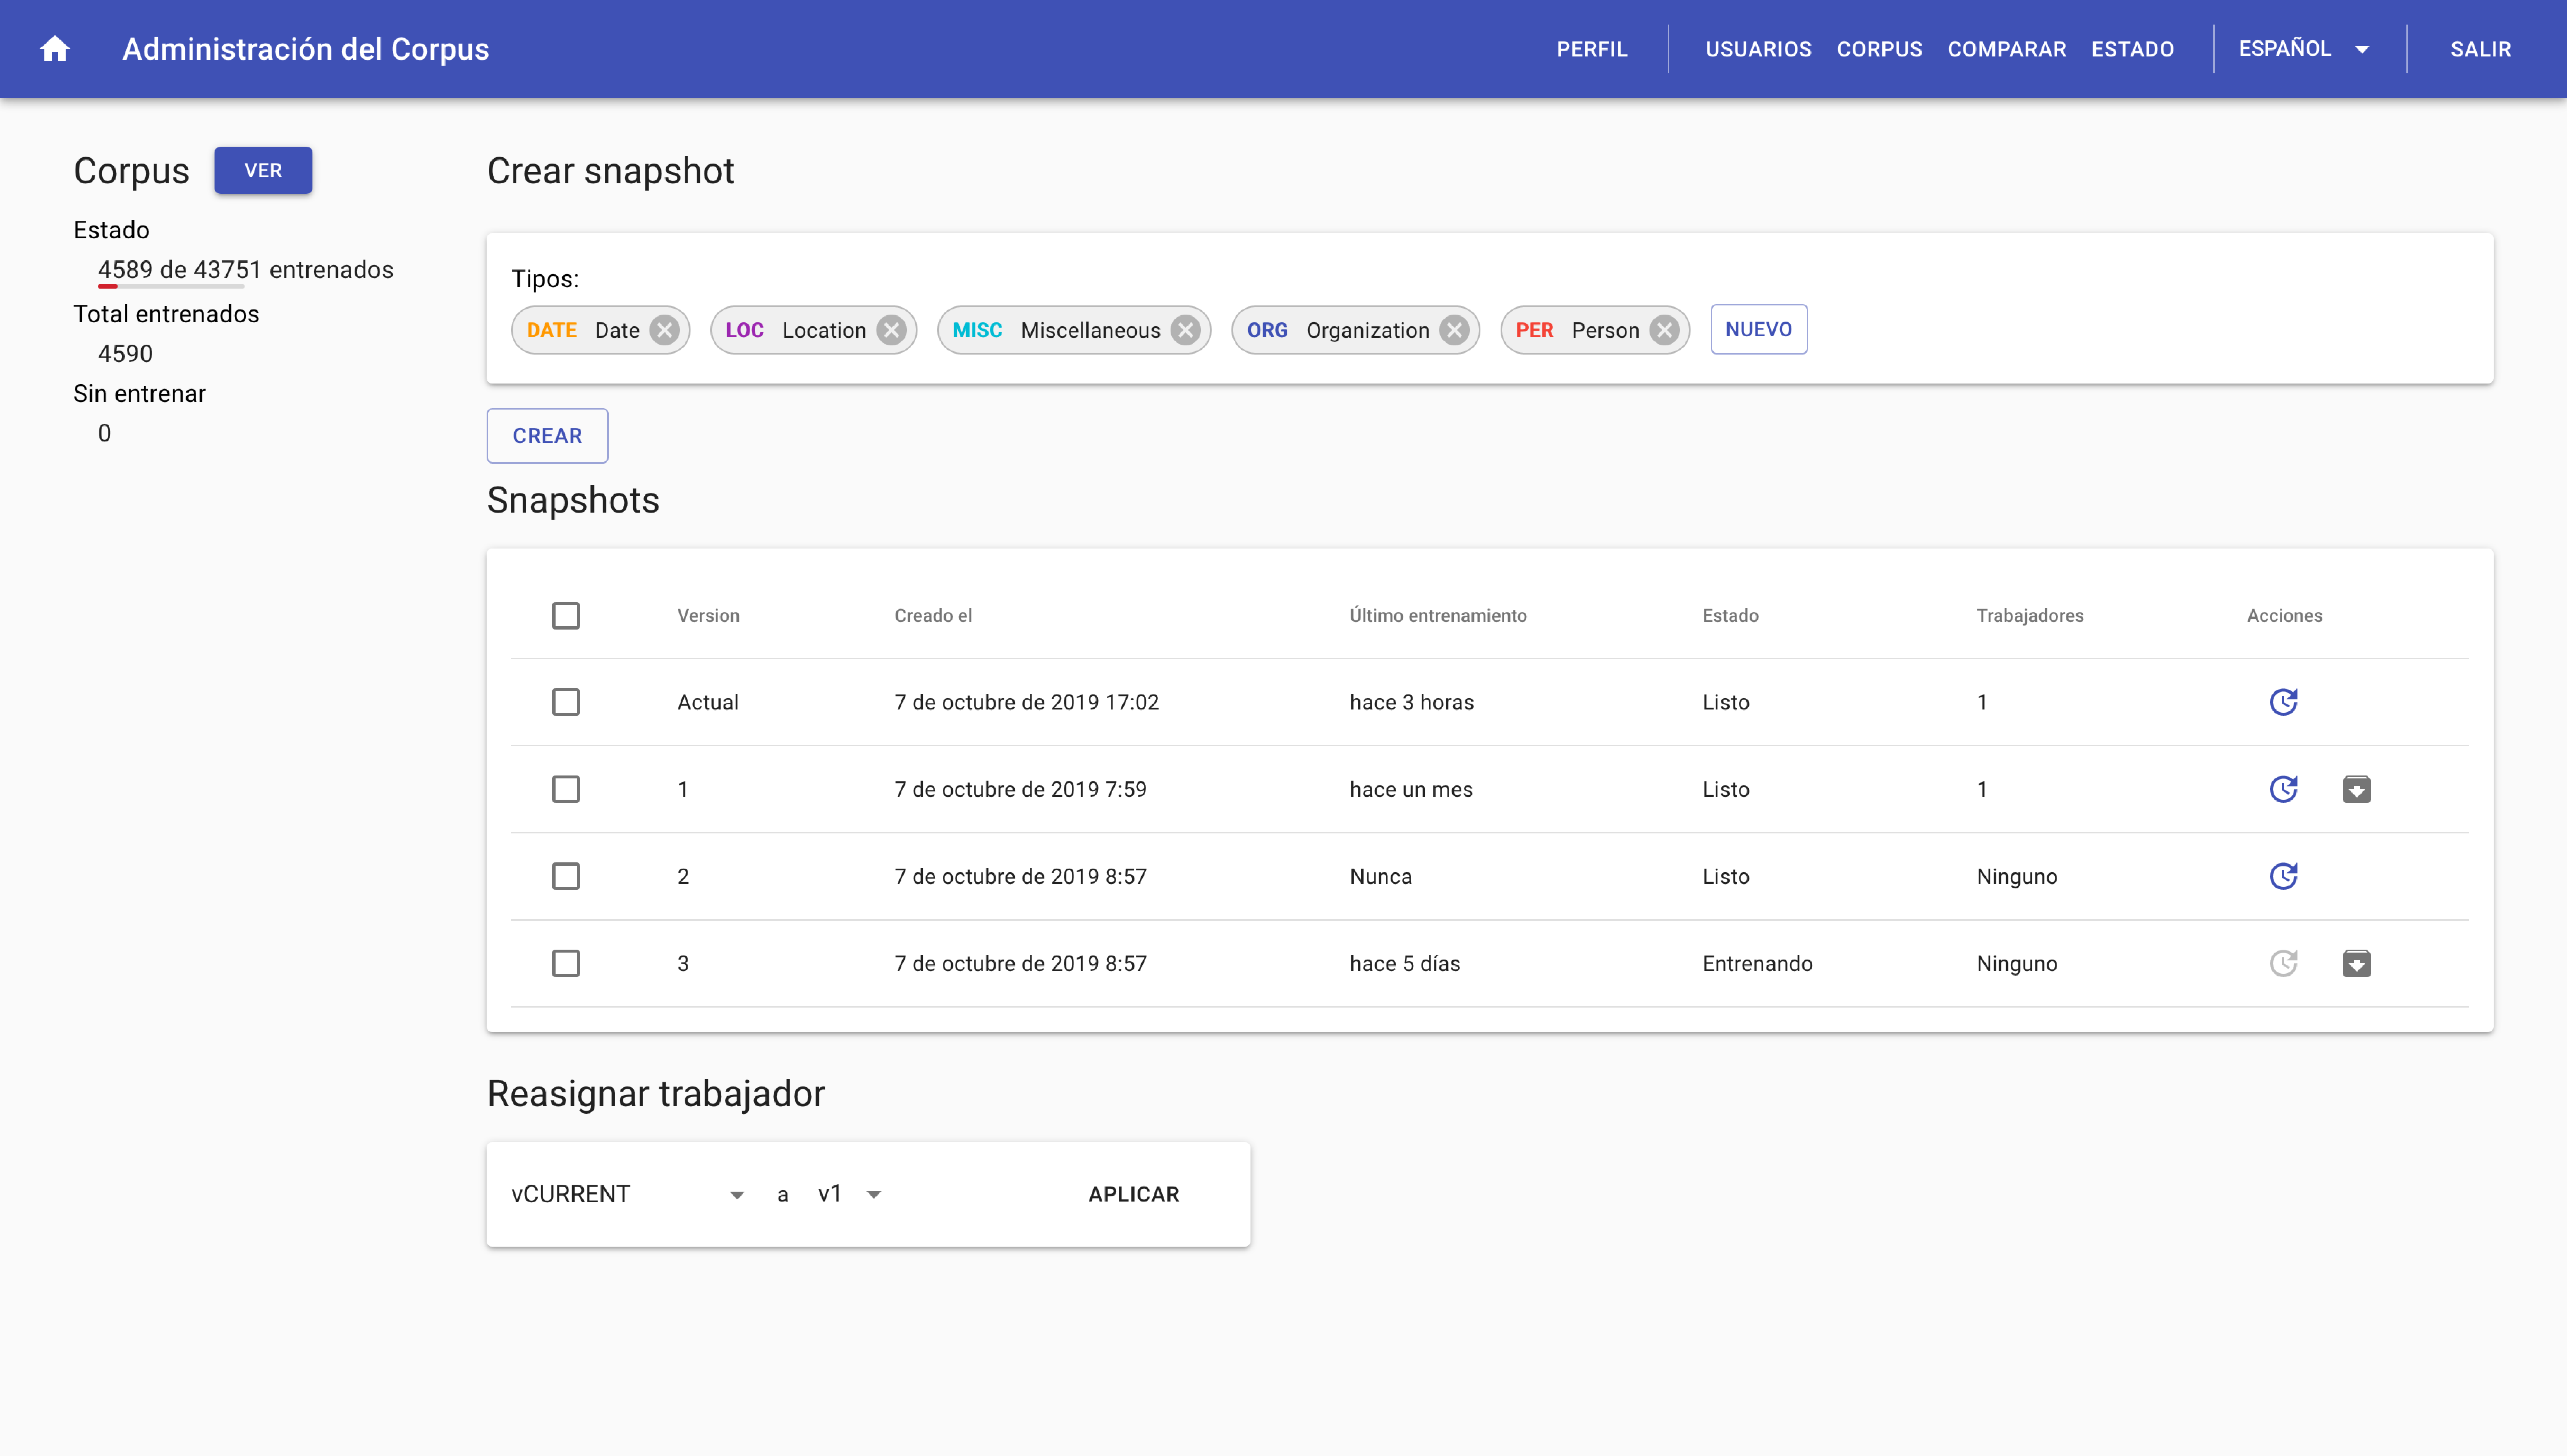
\includegraphics{assets/logic/status.pdf} 

}

\caption{Información de corpus y manejo de workers}\label{fig:logic-status}
\end{figure}

\hypertarget{secciones}{%
\subparagraph{Secciones}\label{secciones}}

Corpus

Es la columna la izquierda y aquí se puede ver rápidamente que porcentaje de el corpus contiene correcciones por usuarios así como también saber la cantidad total de correcciones del sistema (un texto puede tener más de una corrección por distintos usuarios) y también presenta un botón que permite al administrador ir a la pantalla de \emph{Corpus}.

Crear snapshot

Es la sección en la cual será posible crear, borrar o modificar los tipos de entidades reconocidos por el snapshot actual. La acción de editar las entidades genera un snapshot nuevo.

Si el administrador así lo quisiera, puede utilizar esta sección para crear un snapshot nuevo sin editar entidades.

Snapshots

Sección en la cual podemos ver la lista completa de snapshots.
Para cada Snapshot, se muestra cuando fue la última vez que se entrenó así como también cuantos trabajadores tiene asignados. Finalmente es posible desde aquí forzar a entrenar el modelo para ese snapshot en particular y también se presenta la opción para desentrenar, borrando el modelo guardado en el disco.

Reasignar trabajador

Sección que permite reasignar trabajadores para que sirvan un snapshot distinto. De esta manera se pueden servir distintas versiones del modelo de inferencia para poder realizar distintas pruebas sobre los mismos.

\hypertarget{sandbox}{%
\paragraph{Sandbox}\label{sandbox}}

La pantalla de \emph{Sandbox} permite a los usuarios hacer consultas al servicio NERd para poder obtener entidades nombradas a partir de textos arbitrarios.
Adicionalmente, si el usuario tiene el rol de entrenador, podrá corregir las entidades inferidas y agregar el texto con sus correcciones al corpus.

\begin{figure}[H]

{\centering 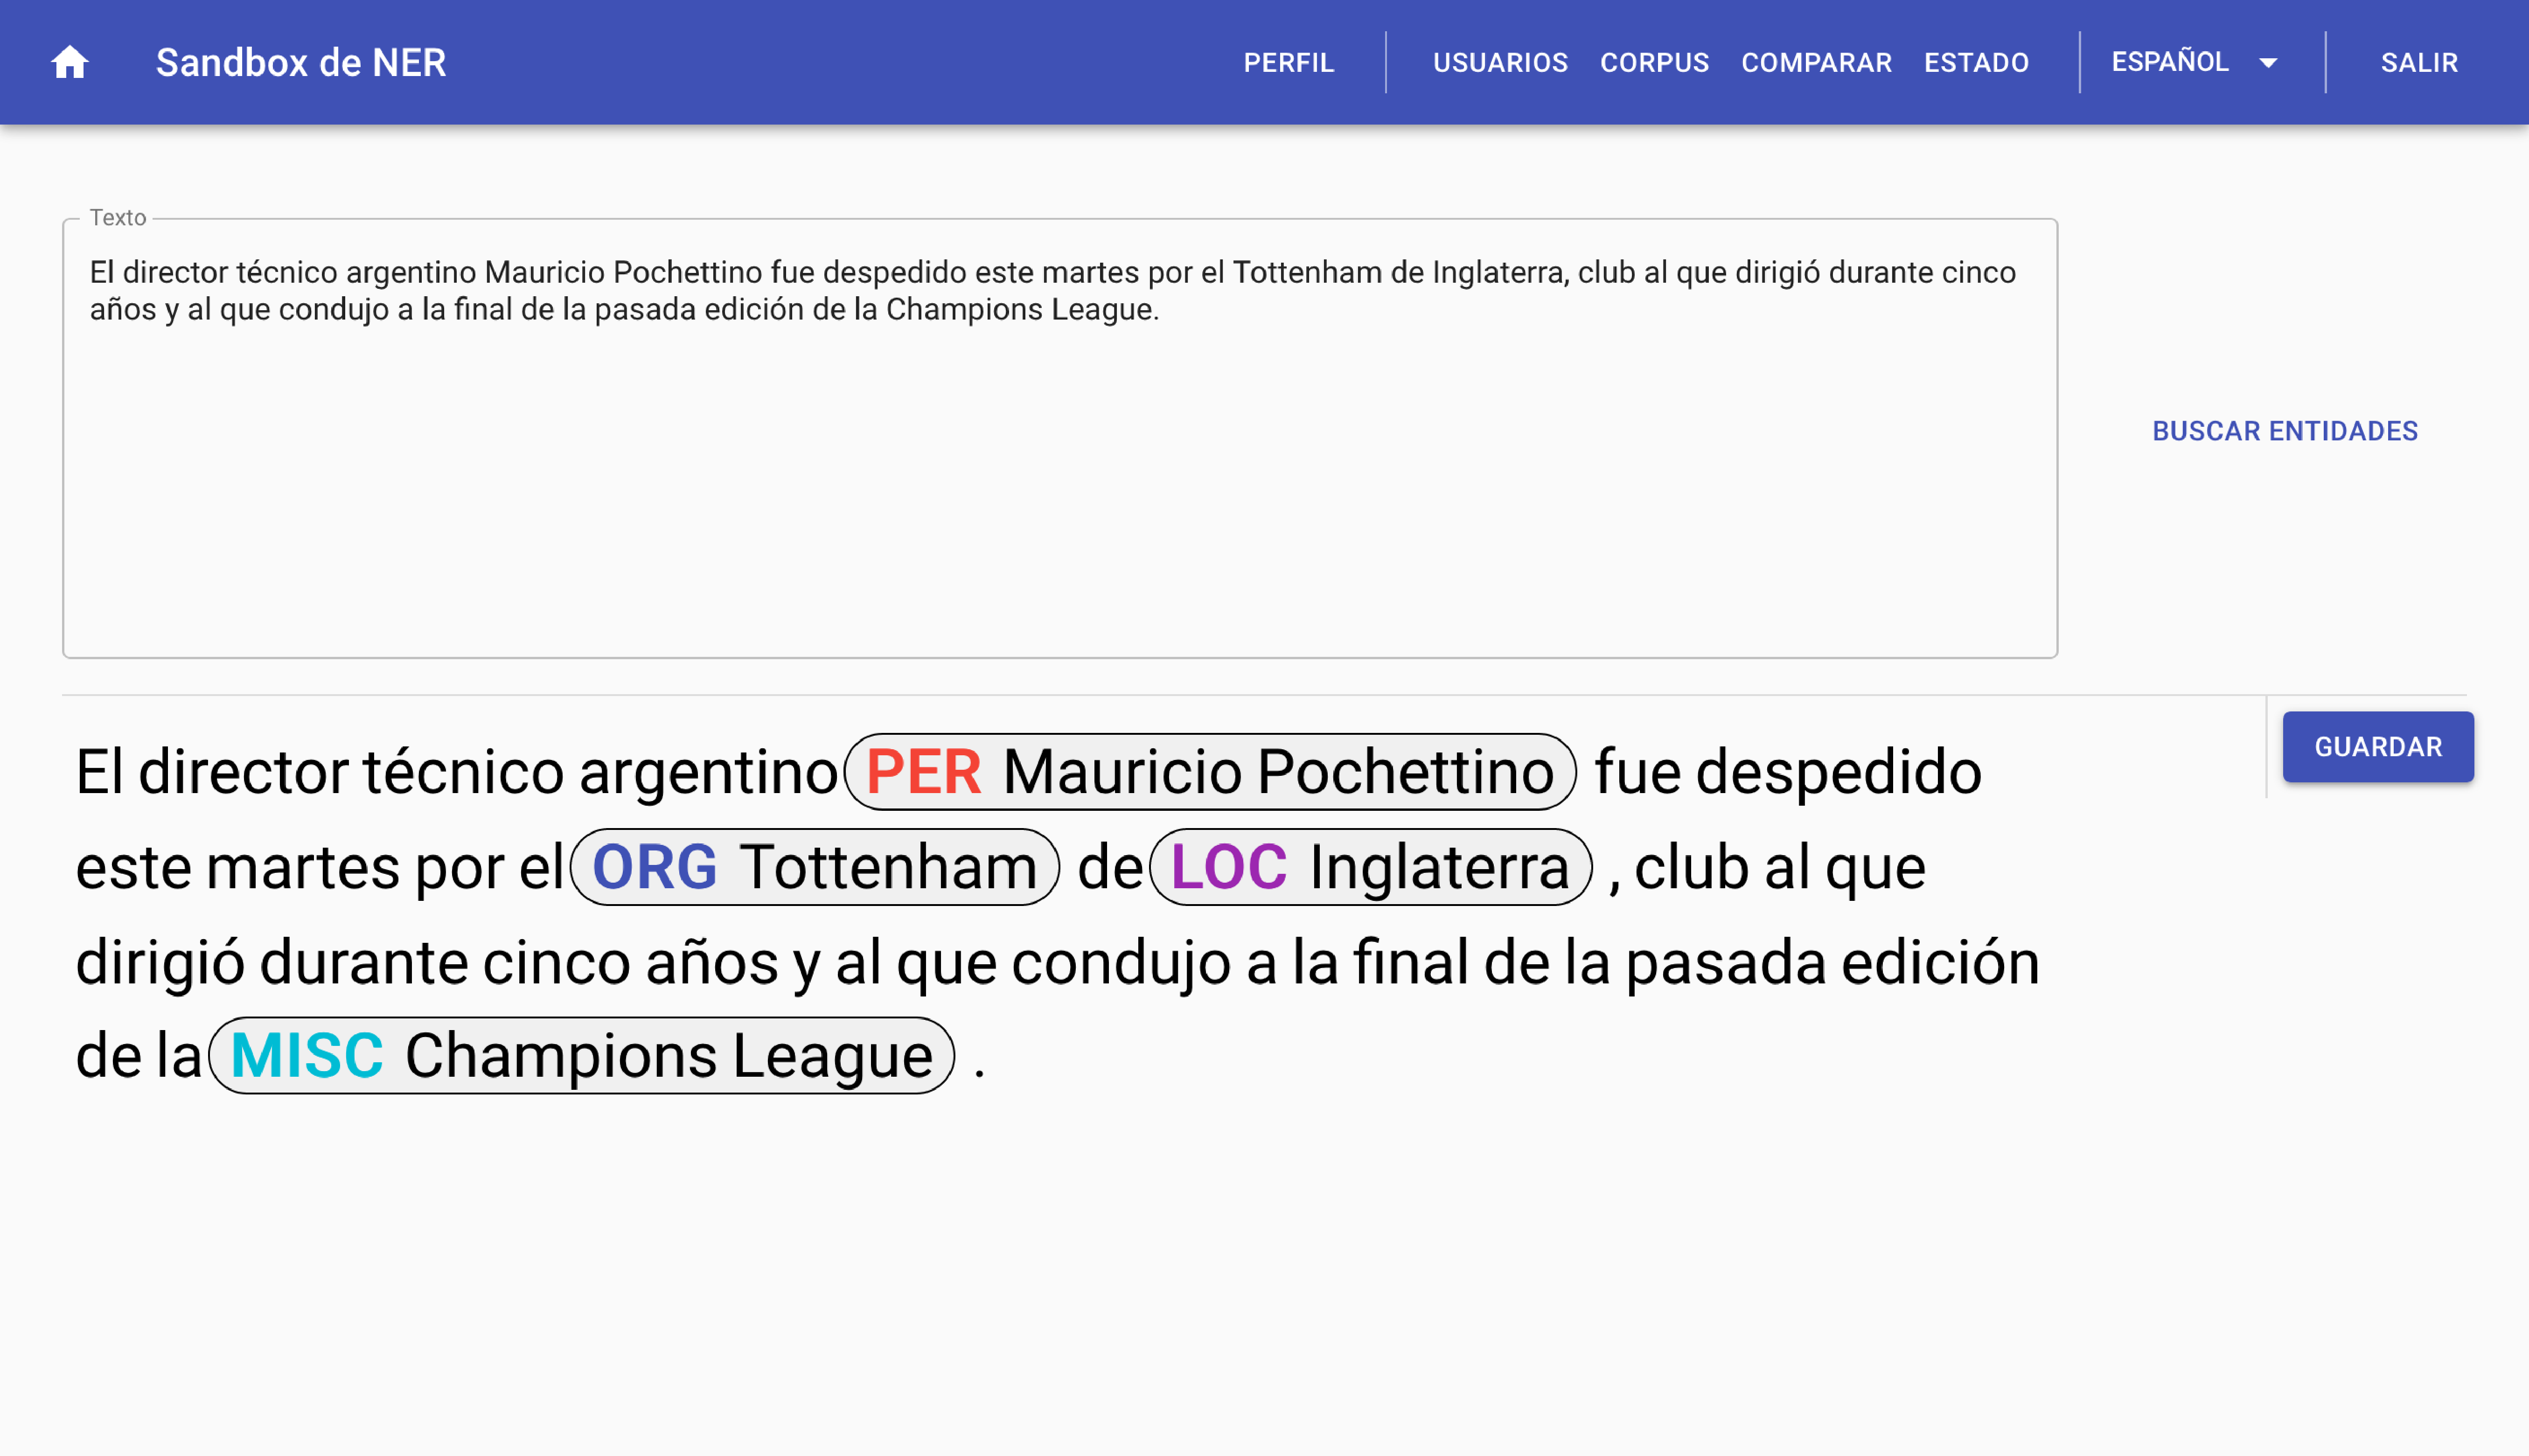
\includegraphics{assets/logic/sandbox.pdf} 

}

\caption{Inferencia de entidades en sandbox}\label{fig:logic-sandbox}
\end{figure}

\hypertarget{comparar}{%
\paragraph{Comparar}\label{comparar}}

Sección accesible únicamente a administradores en la que es posible comparar las entidades inferidas por dos modelos distintos. A su vez, si el usuario logueado tiene el permiso de entrenador, es posible corregir de manera inline los errores en la inferencia del modelo actual.

\begin{figure}[H]

{\centering 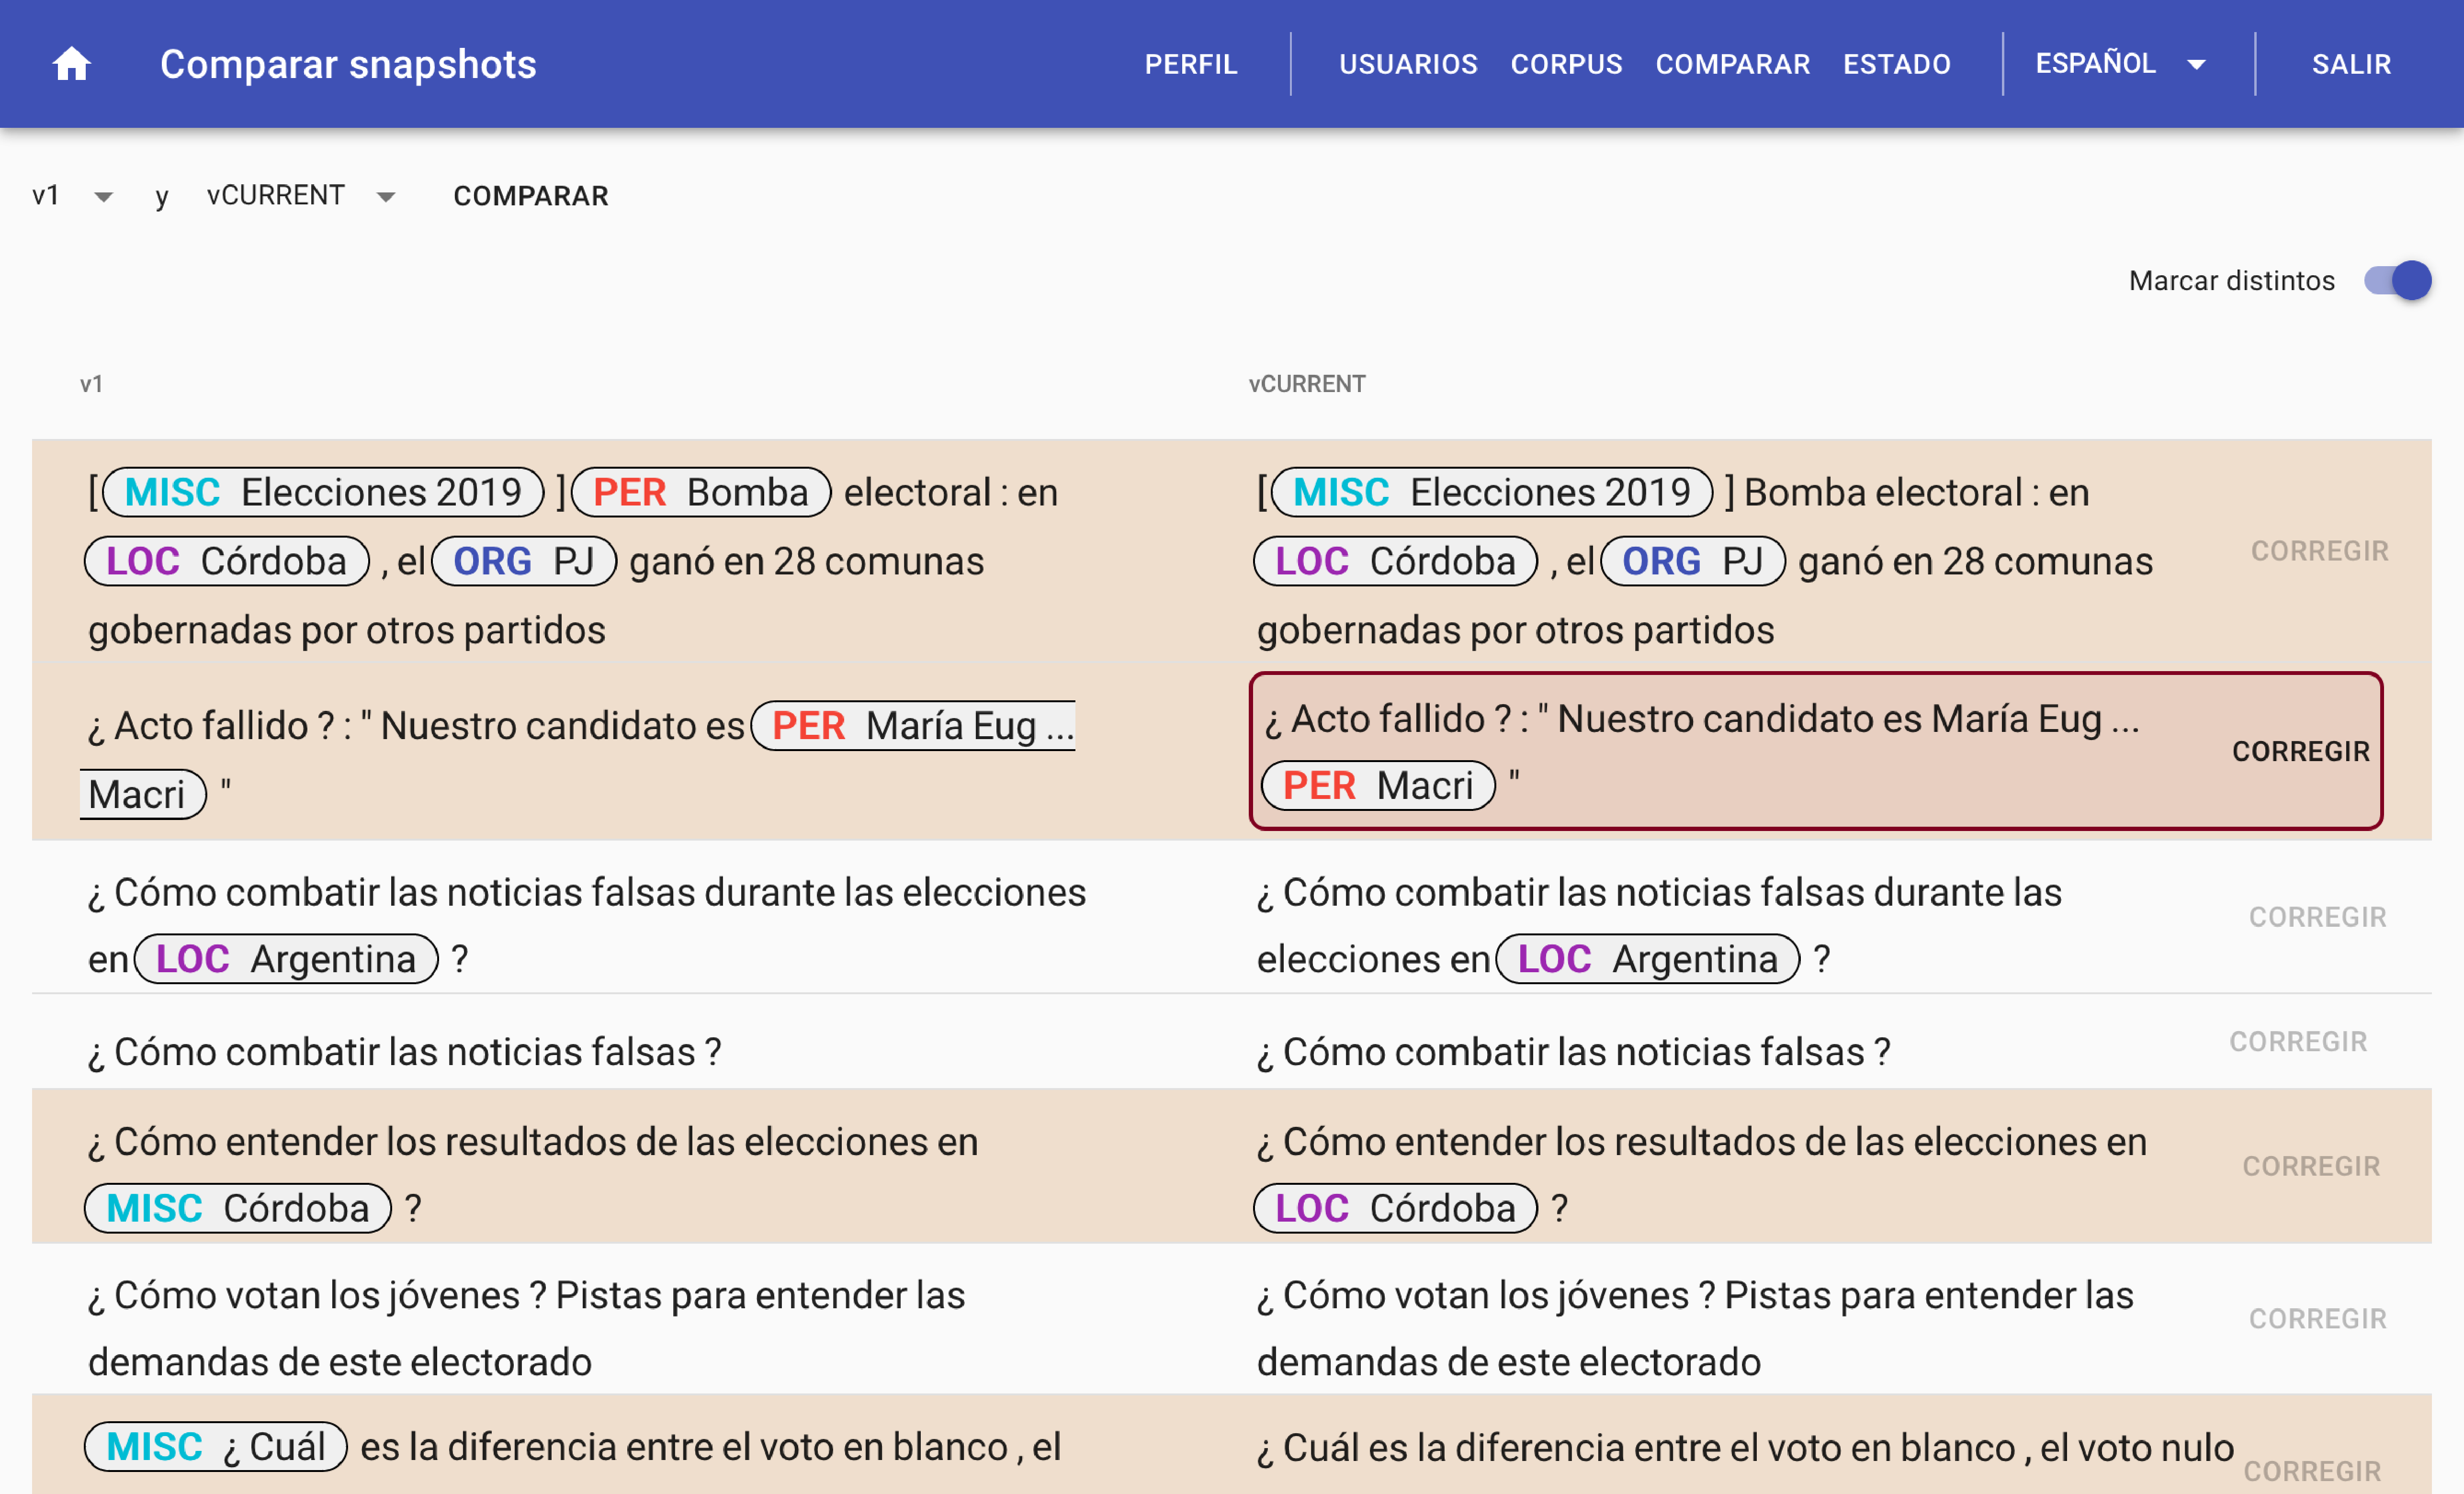
\includegraphics{assets/logic/compare.pdf} 

}

\caption{Comparativa de modelos}\label{fig:logic-compare}
\end{figure}

\hypertarget{vista-de-proceso}{%
\subsection{Vista de proceso}\label{vista-de-proceso}}

\begin{quote}
La vista de proceso trata los aspectos dinámicos del sistema, explica los procesos del sistema y cómo se comunican, y se centra en el comportamiento del sistema en tiempo de ejecución.
La vista de proceso aborda concurrencia, distribución, integradores, rendimiento y escalabilidad, etc.
\end{quote}

\hypertarget{vista-de-desarrollo}{%
\subsection{Vista de desarrollo}\label{vista-de-desarrollo}}

\begin{quote}
La vista de desarrollo ilustra un sistema desde la perspectiva de un programador y se ocupa de la gestión de software.
Esta vista también se conoce como la vista de implementación.
\end{quote}

Python es el lenguaje más utilizado para resolver problemas de Machine Learning, en especial NLP (``The state of the octoverse,'' \protect\hyperlink{ref-github_machine_learning}{2019})

Spacy es el framework mejor ranqueado para la tarea de NLP (``The state of the octoverse,'' \protect\hyperlink{ref-github_machine_learning}{2019}).
Su implementación es robusta y orientada a la implementción de apliciones en producción, a diferencia de muchas otras librerías de NLP que sólo se utilizan con fines académicos.

\hypertarget{vista-fuxedsica}{%
\subsection{Vista física}\label{vista-fuxedsica}}

\begin{quote}
La vista física representa el sistema desde el punto de vista de un ingeniero de sistemas.
Se refiere a la topología de los componentes de software en la capa física, así como a las conexiones físicas entre estos componentes.
Esta vista también se conoce como la vista de \emph{deployment}.
\end{quote}

\hypertarget{escenarios}{%
\subsection{Escenarios}\label{escenarios}}

\begin{quote}
La descripción de una arquitectura se ilustra utilizando un pequeño conjunto de casos de uso, o escenarios, que se convierten en una quinta vista.
Los escenarios describen secuencias de interacciones entre objetos y entre procesos.
Se utilizan para identificar elementos arquitectónicos y para ilustrar y validar el diseño de la arquitectura.
También sirven como punto de partida para las pruebas de un prototipo de arquitectura.
Esta vista también se conoce como vista de caso de uso.
\end{quote}

\hypertarget{results}{%
\section{Resultados}\label{results}}

\hypertarget{discussion}{%
\section{Discusión}\label{discussion}}

\hypertarget{tipos-de-entidades-relevantes}{%
\subsection{Tipos de entidades relevantes}\label{tipos-de-entidades-relevantes}}

tener en cuenta (Brunstein, \protect\hyperlink{ref-brunstein2002}{2002})

\begin{verbatim}
# Notas sobre mejora en tipos de entidades
Presidente -> Person Descriptor
NORP -> (Polical) Peronistas, Kirchneristas
Facility Name -> usually location. "Wall Street", "Muralla China"

Organization Name -> Government vs Corporation.
Product Name -> autos "Fiat Toro", celulares "Galaxy S10"
Events -> Superclásico. Superliga. Copa argentina. Elecciones 2019. Las Paso.
Disease -> 
Game -> Football, Basket (para "titulos" no tan relevante)
\end{verbatim}

\hypertarget{seed-en-los-types}{%
\subsection{Seed en los types}\label{seed-en-los-types}}

en especial para los nuevos.

\hypertarget{mejora-live-vs-offline}{%
\subsection{Mejora live vs offline}\label{mejora-live-vs-offline}}

Mejora \enquote{Uncertainty sampling} -\textgreater{} buscar entidades que tengan un score \textasciitilde{} 0.5

\hypertarget{utilidad-de-la-herramienta}{%
\subsection{Utilidad de la herramienta}\label{utilidad-de-la-herramienta}}

Para poder poner a prueba nuestra herramienta \textbf{NERd} en un entorno real participamos de la hackaton en MediaParty 2019.

\begin{quote}
\textbf{(``Hackaton,'' \protect\hyperlink{ref-hackaton2019}{2019})} es un evento de tres días en Argentina, que reúne a 2500 emprendedores, periodistas, programadores de software y diseñadores de cinco continentes para trabajar juntos para el futuro de los medios de comunicación.
Nacido de Hacks/Hackers Buenos Aires, el evento fusiona a grandes empresas como New York Times, The Guardian, Vox, ProPublica, Watchup, Neo4J o DocumentCloud y comunidades regionales de la mayor red de periodistas y desarrolladores del mundo.
\end{quote}

Participamos en conjunto con otro proyecto final en el que van a utilizar nuestra API para hacer detección de entidades en documentos PDF.

La experiencia fue muy satisfactoria, recibimos buenas críticas sobre la Usabilidad de nuestra aplicación y la gran utilidad que presta a la comunidad.

Por tal motivo recibimos el primer premio de dicha hackaton (``Mención itba,'' \protect\hyperlink{ref-mediaparty2019_win}{2019})

\hypertarget{conclusiones}{%
\section{Conclusiones}\label{conclusiones}}

\hypertarget{examples}{%
\subsection{Examples}\label{examples}}

You can label chapter and section titles using \texttt{\{\#label\}} after them, e.g., we can reference Chapter \ref{intro}. If you do not manually label them, there will be automatic labels anyway, e.g., Chapter \ref{state-of-art}.

Figures and tables with captions will be placed in \texttt{figure} and \texttt{table} environments, respectively.

\begin{Shaded}
\begin{Highlighting}[]
\KeywordTok{par}\NormalTok{(}\DataTypeTok{mar =} \KeywordTok{c}\NormalTok{(}\DecValTok{4}\NormalTok{, }\DecValTok{4}\NormalTok{, }\FloatTok{.1}\NormalTok{, }\FloatTok{.1}\NormalTok{))}
\KeywordTok{plot}\NormalTok{(pressure, }\DataTypeTok{type =} \StringTok{'b'}\NormalTok{, }\DataTypeTok{pch =} \DecValTok{19}\NormalTok{)}
\end{Highlighting}
\end{Shaded}

\begin{figure}

{\centering 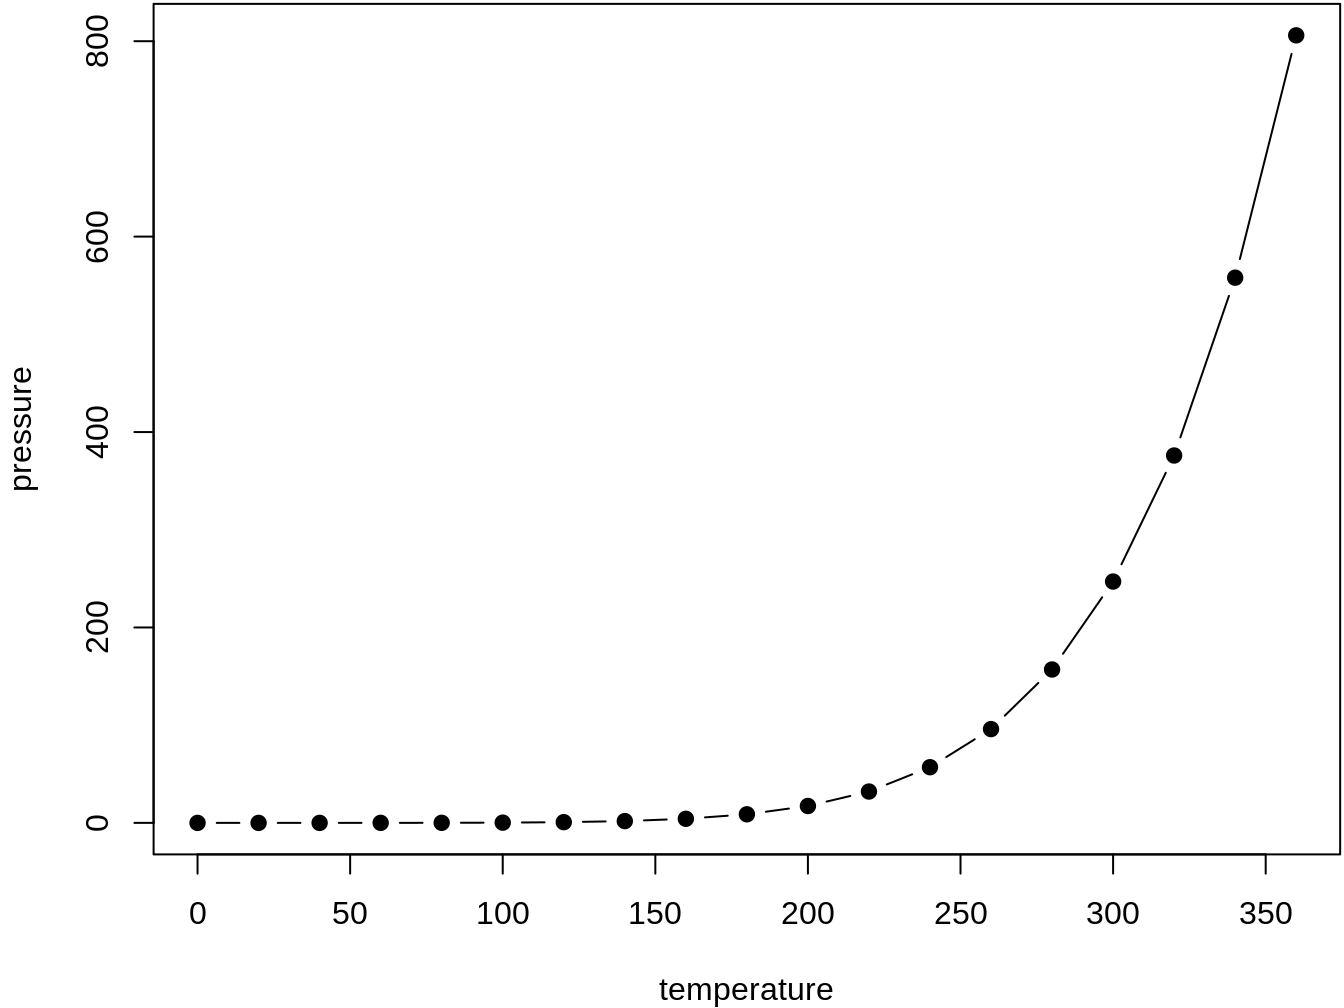
\includegraphics[width=0.8\linewidth]{nerd-pf_files/figure-latex/nice-fig-1.pdf} 

}

\caption{Here is a nice figure!}\label{fig:nice-fig}
\end{figure}

Reference a figure by its code chunk label with the \texttt{fig:} prefix, e.g., see Figure \ref{fig:nice-fig}. Similarly, you can reference tables generated from \texttt{knitr::kable()}, e.g., see Table \ref{tab:nice-tab}.

\begin{Shaded}
\begin{Highlighting}[]
\NormalTok{knitr}\OperatorTok{::}\KeywordTok{kable}\NormalTok{(}
  \KeywordTok{head}\NormalTok{(iris, }\DecValTok{20}\NormalTok{), }\DataTypeTok{caption =} \StringTok{'Here is a nice table!'}\NormalTok{,}
  \DataTypeTok{booktabs =} \OtherTok{TRUE}
\NormalTok{)}
\end{Highlighting}
\end{Shaded}

\begin{table}

\caption{\label{tab:nice-tab}Here is a nice table!}
\centering
\begin{tabular}[t]{rrrrl}
\toprule
Sepal.Length & Sepal.Width & Petal.Length & Petal.Width & Species\\
\midrule
5.1 & 3.5 & 1.4 & 0.2 & setosa\\
4.9 & 3.0 & 1.4 & 0.2 & setosa\\
4.7 & 3.2 & 1.3 & 0.2 & setosa\\
4.6 & 3.1 & 1.5 & 0.2 & setosa\\
5.0 & 3.6 & 1.4 & 0.2 & setosa\\
\addlinespace
5.4 & 3.9 & 1.7 & 0.4 & setosa\\
4.6 & 3.4 & 1.4 & 0.3 & setosa\\
5.0 & 3.4 & 1.5 & 0.2 & setosa\\
4.4 & 2.9 & 1.4 & 0.2 & setosa\\
4.9 & 3.1 & 1.5 & 0.1 & setosa\\
\addlinespace
5.4 & 3.7 & 1.5 & 0.2 & setosa\\
4.8 & 3.4 & 1.6 & 0.2 & setosa\\
4.8 & 3.0 & 1.4 & 0.1 & setosa\\
4.3 & 3.0 & 1.1 & 0.1 & setosa\\
5.8 & 4.0 & 1.2 & 0.2 & setosa\\
\addlinespace
5.7 & 4.4 & 1.5 & 0.4 & setosa\\
5.4 & 3.9 & 1.3 & 0.4 & setosa\\
5.1 & 3.5 & 1.4 & 0.3 & setosa\\
5.7 & 3.8 & 1.7 & 0.3 & setosa\\
5.1 & 3.8 & 1.5 & 0.3 & setosa\\
\bottomrule
\end{tabular}
\end{table}

You can write citations, too. For example, we are using the \textbf{bookdown} package (Xie, \protect\hyperlink{ref-R-bookdown}{2019}) in this sample book, which was built on top of R Markdown and \textbf{knitr} (Xie, \protect\hyperlink{ref-xie2015}{2015}).

\hypertarget{refs}{}
\leavevmode\hypertarget{ref-brunstein2002}{}%
Brunstein, A. (2002). Annotation guidelines for answer types. Retrieved from \url{https://catalog.ldc.upenn.edu/docs/LDC2005T33/BBN-Types-Subtypes.html}

\leavevmode\hypertarget{ref-cambridge_duh}{}%
Duh definition. (2019). Retrieved October 14, 2019, from \url{https://dictionary.cambridge.org/es/diccionario/ingles/duh}

\leavevmode\hypertarget{ref-ethayarajh-etal-2019-towards}{}%
Ethayarajh, K., Duvenaud, D., \& Hirst, G. (2019). Towards understanding linear word analogies. \emph{Proceedings of the 57th annual meeting of the association for computational linguistics}, 3253--3262. \url{https://doi.org/10.18653/v1/P19-1315}

\leavevmode\hypertarget{ref-hackaton2019}{}%
Hackaton. (2019). Retrieved August 31, 2019, from \url{https://mediaparty.info/}

\leavevmode\hypertarget{ref-Kruchten:1995:VMA:624610.625529}{}%
Kruchten, P. (1995). The 4+1 view model of architecture. \emph{IEEE Softw.}, \emph{12}(6), 42--50. \url{https://doi.org/10.1109/52.469759}

\leavevmode\hypertarget{ref-mediaparty2019_win}{}%
Mención itba. (2019). Retrieved October 3, 2019, from \url{https://www.instagram.com/p/B3Koum2peD-/}

\leavevmode\hypertarget{ref-github_machine_learning}{}%
The state of the octoverse: Machine learning. (2019). Retrieved January 24, 2019, from \url{https://github.blog/2019-01-24-the-state-of-the-octoverse-machine-learning/}

\leavevmode\hypertarget{ref-xie2015}{}%
Xie, Y. (2015). \emph{Dynamic documents with R and knitr} (2nd ed.). Retrieved from \url{http://yihui.name/knitr/}

\leavevmode\hypertarget{ref-R-bookdown}{}%
Xie, Y. (2019). \emph{Bookdown: Authoring books and technical documents with r markdown}. Retrieved from \url{https://github.com/rstudio/bookdown}


\end{document}
